\documentclass{article}
\usepackage{newtxtext}
\usepackage{newtxmath}

\usepackage{booktabs} % for better looking tables
\usepackage{graphicx}
\usepackage{caption} % for customizing captions
\usepackage[table]{xcolor} % for coloring tables
\usepackage{pdflscape} % for landscape orientation
\usepackage{arydshln} % for dotted lines in tables	
\usepackage{adjustbox} % For adjusting table position
\usepackage{siunitx}
\usepackage{amsmath}
\usepackage{rotating}
\usepackage{lscape}
\usepackage{multirow}
%\usepackage{geometry}
\usepackage{hhline} % for bold lines
\usepackage{appendix} % for appendix numbering



\begin{document}
	
	
\thispagestyle{empty} % Remove page number from this page
\noindent
APPENDIX A: \newline
CORPORATE DEMOGRAPHY AND WAGE INEQUALITY: REVISITED\newline
2024-05-22
% Summary Statistics
\clearpage % Start a new page
\thispagestyle{empty} % Remove page number from this page


%%% APPENDIX

\appendix
\setcounter{page}{-1}

\setcounter{table}{0}
\renewcommand{\thetable}{A\arabic{table}}

\setcounter{figure}{0}
\renewcommand{\thefigure}{A\arabic{figure}}


\listoftables
\listoffigures
\thispagestyle{empty} % Remove page number from this page

%\clearpage % Start a new page


%\thispagestyle{empty} % Remove page number from this page






%%%%%%%%%%%%%%%%%%%%%%%%%%%
% 1992 - 1998
%%%%%%%%%%%%%%%%%%%%%%%%%%%


\clearpage % Start a new page

%\thispagestyle{empty} % Remove page number from this page
\begin{table}[!htbp] \centering \renewcommand*{\arraystretch}{1.1}\caption{Summary Statistics: 1992 - 1998}\resizebox{\textwidth}{!}{
\begin{tabular}{lrrrrr}
\hline
\hline
Variable & N & Mean & SD & Min & Max \\ 
\hline
Gross wage dispersion & 55295 & 2.03 & 0.512 & -4.95 & 4.92 \\ 
Log mean industry wage & 55295 & 2.52 & 0.44 & -2.16 & 4.19 \\ 
Residual wage dispersion & 55295 & -0.0505 & 0.342 & -1.85 & 1.53 \\ 
Industry employment in township & 55295 & 260 & 1145 & 2 & 65749 \\ 
Total N firms in township (10-3) & 55295 & 0.761 & 1.92 & 0.045 & 25.4 \\ 
Single industry employer & 55295 & 0.157 & 0.363 & 0 & 1 \\ 
Standard deviation of employer sizes & 55295 & 24.6 & 92.5 & 0 & 5026 \\ 
Log N industry firms in township & 55295 & 1.86 & 1.38 & 0 & 8.8 \\ 
N industries in township & 55295 & 28.7 & 5.82 & 11 & 45 \\ 
Entropy of industry shares & 55295 & 2.6 & 0.301 & 1.05 & 3.16 \\ 
Ratio of foreign owned firms in industry-township & 55295 & 0.00159 & 0.0266 & 0 & 1 \\ 
Ratio of non-profit making firms in industry-township & 55295 & 0.0641 & 0.173 & 0 & 1\\ 
\hline
\hline
\end{tabular}
}
\end{table}

 



% Correlation Matrix

\begin{landscape}
% Table 2a
\clearpage % Start a new page

% latex table generated in R 4.0.2 by xtable 1.8-4 package
% Wed Mar 13 17:04:42 2024
\begin{table}[htb]
\centering
\caption{Correlation Matrix 1992 - 1998} 
\begin{tabular}{lrrrrrrrrrrr}
  \hline
 & 1 & 2 & 3 & 4 & 5 & 6 & 7 & 8 & 9 & 10 & 11 \\ 
  \hline
Gross wage dispersion &  &  &  &  &  &  &  &  &  &  &  \\ 
  Log mean industry wage & 0.58 &  &  &  &  &  &  &  &  &  &  \\ 
  Residual wage dispersion & 0.28 & -0.33 &  &  &  &  &  &  &  &  &  \\ 
  Industry employment in township & 0.13 & 0.09 & 0.00 &  &  &  &  &  &  &  &  \\ 
  Total N firms in township (10-3) & 0.17 & 0.14 & 0.00 & 0.50 &  &  &  &  &  &  &  \\ 
  Single industry employer & -0.27 & -0.09 & -0.17 & -0.08 & -0.07 &  &  &  &  &  &  \\ 
  Standard deviation of employer sizes & 0.10 & 0.16 & -0.10 & 0.27 & 0.07 & -0.11 &  &  &  &  &  \\ 
  Log N industry firms in township & 0.25 & 0.04 & 0.21 & 0.36 & 0.28 & -0.58 & 0.03 &  &  &  &  \\ 
  N industries in township & 0.23 & 0.23 & -0.01 & 0.24 & 0.48 & -0.12 & 0.10 & 0.32 &  &  &  \\ 
  Entropy of industry shares & 0.14 & 0.13 & 0.01 & 0.10 & 0.22 & -0.09 & 0.00 & 0.20 & 0.64 &  &  \\ 
  Ratio of foreign owned firms in industry-township & 0.04 & 0.05 & -0.02 & 0.03 & 0.13 & -0.01 & 0.02 & 0.01 & 0.06 & 0.02 &  \\ 
  Ratio of non-profit making firms in industry-township & 0.06 & -0.10 & 0.22 & -0.02 & -0.03 & -0.03 & -0.05 & 0.04 & -0.05 & -0.02 & -0.01 \\ 
   \hline
\end{tabular}
\end{table}
 % Include the first table
\end{landscape}



% Main tables: models

\clearpage % Start a new page
%\thispagestyle{empty} % Remove page number from this page

\begin{table}[htbp]
\centering
\caption{Estimated Effects of Regional Corporate Demography on Gross Income Dispersion in an Industry-Township,  1992 to 1998}
\resizebox{\linewidth}{!}{%
   \begingroup
\centering
\begin{tabular}{lccccc}
   \tabularnewline \multicolumn{6}{c}{\textit{DV: Gross Income Dispersion}} \\ \midrule \midrule
   Model:                               & (1)              & (2)              & (3)              & (4)              & (5)\\  
   \midrule
   \emph{Variables}\\
   Log mean industry wage               & 659.119$^{***}$  & 660.009$^{***}$  & 659.096$^{***}$  & 658.600$^{***}$  & 658.193$^{***}$\\   
                                        & (15.950)         & (16.112)         & (16.042)         & (16.127)         & (16.049)\\   
   Industry employment in township      & -0.007$^{***}$   & -0.008$^{***}$   & -0.007$^{***}$   & -0.004$^{**}$    & -0.007$^{***}$\\   
                                        & (0.001)          & (0.001)          & (0.001)          & (0.001)          & (0.001)\\   
   Total N firms in township (10-3)     & 12.232$^{***}$   & 13.131$^{***}$   & 12.294$^{***}$   & 15.238$^{***}$   & 12.489$^{***}$\\   
                                        & (1.256)          & (1.160)          & (1.164)          & (1.001)          & (1.077)\\   
\hdashline % Dotted line
\\[0.1ex] % Add space of 1ex between rows
\emph{H1} \\ 
   Single industry employer             & -199.402$^{***}$ & -197.002$^{***}$ & -198.814$^{***}$ & -179.566$^{***}$ & -190.190$^{***}$\\   
                                        & (12.531)         & (12.860)         & (12.732)         & (13.018)         & (12.989)\\   
   Log N industry firms in township     & 54.971$^{***}$   & 60.835$^{***}$   & 57.664$^{***}$   & 123.369$^{***}$  & 128.579$^{***}$\\   
                                        & (3.744)          & (4.457)          & (4.178)          & (12.921)         & (18.546)\\   
\hdashline % Dotted line
\\[0.1ex] % Add space of 1ex between rows
\emph{H2} \\ 
   Standard deviation of employer sizes &                  & -0.001           & -0.005           & -0.012           & -0.007\\   
                                        &                  & (0.026)          & (0.026)          & (0.025)          & (0.025)\\   
   N industries in township             &                  & -1.502$^{*}$     &                  & 1.171            &   \\   
                                        &                  & (0.690)          &                  & (1.089)          &   \\   
   Entropy of industry shares           &                  &                  & -18.176          &                  & 21.602\\   
                                        &                  &                  & (10.838)         &                  & (16.936)\\   
\hdashline % Dotted line
\\[0.1ex] % Add space of 1ex between rows
\emph{H3} \\ 
   Log N firms X N industries           &                  &                  &                  & -1.860$^{***}$   &   \\   
                                        &                  &                  &                  & (0.396)          &   \\   
   Log N firms X entropy                &                  &                  &                  &                  & -25.610$^{***}$\\   
                                        &                  &                  &                  &                  & (6.640)\\   
   \midrule
   \emph{Fixed-effects}\\
   Industry                             & Yes              & Yes              & Yes              & Yes              & Yes\\  
   Year                                 & Yes              & Yes              & Yes              & Yes              & Yes\\  
   \midrule
   \emph{Fit statistics}\\
   R$^2$                                & 0.454            & 0.455            & 0.455            & 0.455            & 0.455\\  
   Within R$^2$                         & 0.362            & 0.362            & 0.362            & 0.363            & 0.362\\  
   Observations                         & 55,295           & 55,295           & 55,295           & 55,295           & 55,295\\  
   \midrule \midrule
\multicolumn{6}{p{16cm}}{\emph{Notes:} The dependent variable is the log 
    standard deviation of the yearly income from the largest workplace for 
    employees in a given industry in a township, multiplied by 1,000. Standard 
    errors are adjusted for clustering at the township level. Models include 
    dummy variables for year and industry. Interaction effects are centered. 
    Clustered (Township) standard-errors in parentheses.}\\
\multicolumn{6}{l}{\emph{*** p$<$0.001, ** p$<$0.01, * p$<$0.05}} \\ 
\end{tabular}
\par\endgroup
 % Assuming table_grosswage_extension_1998.tex contains your table
   }
    \captionsetup{justification=centering,  font=small} % Centering the caption
    \label{appendix:yourlabel}
\end{table}

\clearpage % Start a new page
%\thispagestyle{empty} % Remove page number from this page

\begin{table}[htbp]

    \centering
        \caption{Estimated Effects of Regional Corporate Demography on Residual Income Dispersion in an Industry-Township,  1992 to 1998}
    \resizebox{\linewidth}{!}{%
        \begingroup
\centering
\begin{tabular}{lccccc}
   \tabularnewline \multicolumn{6}{c}{\textit{DV: Residual Income Dispersion}} \\ \midrule \midrule
   Model:                               & (1)             & (2)             & (3)             & (4)             & (5)\\  
   \midrule
   \emph{Variables}\\
   Industry employment in township      & -0.010          & -0.005          & -0.004          & -0.004          & -0.003\\   
                                        & (0.006)         & (0.003)         & (0.002)         & (0.003)         & (0.002)\\   
   Total N firms in township (10-3)     & 0.962           & 1.121           & -0.537          & 1.697$^{**}$    & -0.522\\   
                                        & (0.600)         & (0.641)         & (0.775)         & (0.604)         & (0.773)\\   
\hdashline % Dotted line
\\[0.1ex] % Add space of 1ex between rows
\emph{H1} \\ 
   Single industry employer             & -64.719$^{***}$ & -72.511$^{***}$ & -76.869$^{***}$ & -67.707$^{***}$ & -76.161$^{***}$\\   
                                        & (8.805)         & (9.157)         & (8.988)         & (9.509)         & (9.067)\\   
   Log N industry firms in township     & 15.169$^{***}$  & 26.326$^{***}$  & 15.889$^{***}$  & 43.450$^{***}$  & 21.676\\   
                                        & (3.364)         & (3.762)         & (3.336)         & (9.989)         & (15.165)\\   
\hdashline % Dotted line
\\[0.1ex] % Add space of 1ex between rows
\emph{H2} \\ 
   Standard deviation of employer sizes &                 & -0.233$^{***}$  & -0.236$^{***}$  & -0.236$^{***}$  & -0.236$^{***}$\\   
                                        &                 & (0.044)         & (0.043)         & (0.044)         & (0.043)\\   
   N industries in township             &                 & -2.733$^{***}$  &                 & -2.002$^{*}$    &   \\   
                                        &                 & (0.591)         &                 & (0.884)         &   \\   
   Entropy of industry shares           &                 &                 & -2.497          &                 & 0.754\\   
                                        &                 &                 & (9.384)         &                 & (16.202)\\   
\hdashline % Dotted line
\\[0.1ex] % Add space of 1ex between rows
\emph{H3} \\ 
   Log N firms X N industries           &                 &                 &                 & -0.510          &   \\   
                                        &                 &                 &                 & (0.297)         &   \\   
   Log N firms X entropy                &                 &                 &                 &                 & -2.092\\   
                                        &                 &                 &                 &                 & (5.582)\\   
   \midrule
   \emph{Fixed-effects}\\
   Industry                             & Yes             & Yes             & Yes             & Yes             & Yes\\  
   Year                                 & Yes             & Yes             & Yes             & Yes             & Yes\\  
   \midrule
   \emph{Fit statistics}\\
   R$^2$                                & 0.183           & 0.188           & 0.187           & 0.188           & 0.187\\  
   Within R$^2$                         & 0.009           & 0.015           & 0.013           & 0.015           & 0.013\\  
   Observations                         & 55,295          & 55,295          & 55,295          & 55,295          & 55,295\\  
   \midrule \midrule
\multicolumn{6}{p{16cm}}{\emph{Notes:} The dependent variable is the log 
    standard deviation of the residuals from the first-stage human capital equation 
    regressions adjusted for sampling error, multiplied by 1,000. Standard errors 
    are adjusted for clustering at the township level. Models include dummy variables 
    for year and industry. Interaction effects are centered. Clustered (Township) 
    standard-errors in parentheses.}\\
\multicolumn{6}{l}{\emph{*** p$<$0.001, ** p$<$0.01, * p$<$0.05}} \\ 
\end{tabular}
\par\endgroup
 % Assuming table_grosswage_extension_1998.tex contains your table
    }
     \captionsetup{justification=centering,  font=small} % Centering the caption

    \label{tab:yourlabel}
\end{table}


\clearpage % Start a new page


\begin{landscape}
%\thispagestyle{empty} % Remove page number from this page
\begin{table}[t] % Change the placement specifier from [htbp] to [t]
\vspace*{-2cm} % Adjust the space between the top of the page and the table
\centering
\caption{Extended Models of Corporate Demography (Foreign and Non-profit Firms) on Gross Income Dispersion, 1992-1998}
\resizebox{\linewidth}{!}{%
    \begingroup
\centering
\begin{tabular}{lcccccccc}
   \tabularnewline \multicolumn{9}{c}{\textit{DV: Gross Income Dispersion}} \\ \midrule \midrule
   Model:                                                & (1)             & (2)             & (3)             & (4)              & (5)              & (6)              & (7)              & (8)\\  
   \midrule
   \emph{Variables}\\
   Log mean industry wage                                & 716.184$^{***}$ & 717.670$^{***}$ & 717.330$^{***}$ & 660.851$^{***}$  & 661.688$^{***}$  & 660.870$^{***}$  & 660.280$^{***}$  & 659.968$^{***}$\\   
                                                         & (16.037)        & (16.172)        & (16.208)        & (16.160)         & (16.319)         & (16.256)         & (16.337)         & (16.264)\\   
   Industry employment in township                       & 0.000           & 0.000           & 0.000           & -0.007$^{***}$   & -0.008$^{***}$   & -0.007$^{***}$   & -0.003$^{**}$    & -0.007$^{***}$\\   
                                                         & (0.003)         & (0.003)         & (0.003)         & (0.001)          & (0.001)          & (0.001)          & (0.001)          & (0.001)\\   
   Total N firms in township (10-3)                      & 26.819$^{***}$  & 26.989$^{***}$  & 26.857$^{***}$  & 12.240$^{***}$   & 13.099$^{***}$   & 12.296$^{***}$   & 15.206$^{***}$   & 12.495$^{***}$\\   
                                                         & (4.116)         & (4.145)         & (4.139)         & (1.252)          & (1.161)          & (1.164)          & (0.999)          & (1.076)\\   
\hdashline % Dotted line
\\[0.1ex] % Add space of 1ex between rows
\emph{H4} \\ 
   Ratio of foreign owned firms in industry-township     & 134.279         &                 & 133.575         & 46.199           & 40.957           & 41.685           & 37.500           & 37.891\\   
                                                         & (109.401)       &                 & (109.393)       & (87.366)         & (87.196)         & (86.938)         & (86.887)         & (85.790)\\   
   Ratio of non-profit making firms in industry-township &                 & 30.753          & 30.616          & 51.036           & 49.360           & 51.130           & 49.139           & 50.884\\   
                                                         &                 & (37.498)        & (37.494)        & (37.197)         & (37.156)         & (37.189)         & (37.082)         & (37.195)\\   
\hdashline % Dotted line
\\[0.1ex] % Add space of 1ex between rows
\emph{H1} \\ 
   Single industry employer                              &                 &                 &                 & -199.828$^{***}$ & -197.579$^{***}$ & -199.317$^{***}$ & -180.167$^{***}$ & -190.719$^{***}$\\   
                                                         &                 &                 &                 & (12.485)         & (12.802)         & (12.684)         & (12.978)         & (12.939)\\   
   Log N industry firms in township                      &                 &                 &                 & 54.966$^{***}$   & 60.609$^{***}$   & 57.651$^{***}$   & 123.059$^{***}$  & 128.364$^{***}$\\   
                                                         &                 &                 &                 & (3.741)          & (4.458)          & (4.175)          & (12.961)         & (18.587)\\   
\hdashline % Dotted line
\\[0.1ex] % Add space of 1ex between rows
\emph{H2} \\ 
   Standard deviation of employer sizes                  &                 &                 &                 &                  & -0.002           & -0.007           & -0.014           & -0.008\\   
                                                         &                 &                 &                 &                  & (0.026)          & (0.026)          & (0.025)          & (0.025)\\   
   N industries in township                              &                 &                 &                 &                  & -1.446$^{*}$     &                  & 1.223            &   \\   
                                                         &                 &                 &                 &                  & (0.689)          &                  & (1.086)          &   \\   
   Entropy of industry shares                            &                 &                 &                 &                  &                  & -18.113          &                  & 21.542\\   
                                                         &                 &                 &                 &                  &                  & (10.869)         &                  & (16.973)\\   
\hdashline % Dotted line
\\[0.1ex] % Add space of 1ex between rows
\emph{H3} \\ 
   Log N firms X N industries                            &                 &                 &                 &                  &                  &                  & -1.858$^{***}$   &   \\   
                                                         &                 &                 &                 &                  &                  &                  & (0.396)          &   \\   
   Log N firms X entropy                                 &                 &                 &                 &                  &                  &                  &                  & -25.536$^{***}$\\   
                                                         &                 &                 &                 &                  &                  &                  &                  & (6.653)\\   
   \midrule
   \emph{Fixed-effects}\\
   Industry                                              & Yes             & Yes             & Yes             & Yes              & Yes              & Yes              & Yes              & Yes\\  
   Year                                                  & Yes             & Yes             & Yes             & Yes              & Yes              & Yes              & Yes              & Yes\\  
   \midrule
   \emph{Fit statistics}\\
   R$^2$                                                 & 0.423           & 0.423           & 0.423           & 0.455            & 0.455            & 0.455            & 0.455            & 0.455\\  
   Within R$^2$                                          & 0.325           & 0.325           & 0.325           & 0.362            & 0.362            & 0.362            & 0.363            & 0.363\\  
   Observations                                          & 55,295          & 55,295          & 55,295          & 55,295           & 55,295           & 55,295           & 55,295           & 55,295\\  
   \midrule \midrule
\multicolumn{9}{p{24cm}}{\emph{Notes:} The dependent variable is the log 
    standard deviation of the yearly income from the largest workplace for 
    employees in a given industry in a township, multiplied by 1,000. Standard 
    errors are adjusted for clustering at the township level. Models include 
    dummy variables for year and industry. Interaction effects are centered. 
    Clustered (Township) standard-errors in parentheses.}\\
\multicolumn{9}{l}{\emph{*** p$<$0.001, ** p$<$0.01, * p$<$0.05}} \\ 
\end{tabular}
\par\endgroup
 % Assuming table4.tex contains your table
}
\captionsetup{justification=centering, font=small} % Centering the caption
\label{tab:yourlabel}
\end{table}
\end{landscape}



\clearpage % Start a new page

\begin{landscape}
%\thispagestyle{empty} % Remove page number from this page
\begin{table}[t] % Change the placement specifier from [htbp] to [t]
\vspace*{-2cm} % Adjust the space between the top of the page and the table
\centering
\caption{Extended Models of Corporate Demography (Foreign and Non-profit Firms) on Residual Income Dispersion, 1992-1998}
\resizebox{\linewidth}{!}{%
    \begingroup
\centering
\begin{tabular}{lcccccccc}
   \tabularnewline \multicolumn{9}{c}{\textit{DV: Residual Income Dispersion}} \\ \midrule \midrule
   Model:                                                & (1)            & (2)             & (3)             & (4)              & (5)             & (6)             & (7)             & (8)\\  
   \midrule
   \emph{Variables}\\
   Industry employment in township                       & -0.007         & -0.007          & -0.007          & -0.010           & -0.005          & -0.004          & -0.004          & -0.003\\   
                                                         & (0.004)        & (0.004)         & (0.004)         & (0.006)          & (0.003)         & (0.002)         & (0.003)         & (0.002)\\   
   Total N firms in township (10-3)                      & 5.821$^{**}$   & 6.290$^{**}$    & 6.450$^{**}$    & 1.487$^{*}$      & 1.415$^{*}$     & -0.035          & 2.011$^{**}$    & -0.017\\   
                                                         & (1.994)        & (2.282)         & (2.265)         & (0.712)          & (0.684)         & (0.645)         & (0.649)         & (0.642)\\   
\hdashline % Dotted line
\\[0.1ex] % Add space of 1ex between rows
\emph{H5} \\ 
   Ratio of foreign owned firms in industry-township     & -151.929$^{*}$ &                 & -152.526$^{*}$  & -191.181$^{***}$ & -187.994$^{**}$ & -180.491$^{**}$ & -189.159$^{**}$ & -180.867$^{**}$\\   
                                                         & (62.261)       &                 & (62.069)        & (57.024)         & (59.023)        & (59.678)        & (59.131)        & (59.628)\\   
   Ratio of non-profit making firms in industry-township &                & 297.002$^{***}$ & 297.016$^{***}$ & 310.450$^{***}$  & 308.588$^{***}$ & 311.867$^{***}$ & 308.657$^{***}$ & 311.872$^{***}$\\   
                                                         &                & (27.260)        & (27.266)        & (26.974)         & (26.906)        & (27.012)        & (26.907)        & (27.014)\\   
\hdashline % Dotted line
\\[0.1ex] % Add space of 1ex between rows
\emph{H1} \\ 
   Single industry employer                              &                &                 &                 & -68.650$^{***}$  & -77.111$^{***}$ & -80.919$^{***}$ & -72.146$^{***}$ & -80.145$^{***}$\\   
                                                         &                &                 &                 & (8.737)          & (9.090)         & (8.942)         & (9.496)         & (9.037)\\   
   Log N industry firms in township                      &                &                 &                 & 16.322$^{***}$   & 26.117$^{***}$  & 17.134$^{***}$  & 43.822$^{***}$  & 23.468\\   
                                                         &                &                 &                 & (3.289)          & (3.702)         & (3.277)         & (9.800)         & (14.810)\\   
\hdashline % Dotted line
\\[0.1ex] % Add space of 1ex between rows
\emph{H2} \\ 
   Standard deviation of employer sizes                  &                &                 &                 &                  & -0.236$^{***}$  & -0.238$^{***}$  & -0.239$^{***}$  & -0.239$^{***}$\\   
                                                         &                &                 &                 &                  & (0.044)         & (0.044)         & (0.044)         & (0.044)\\   
   N industries in township                              &                &                 &                 &                  & -2.390$^{***}$  &                 & -1.634          &   \\   
                                                         &                &                 &                 &                  & (0.576)         &                 & (0.846)         &   \\   
   Entropy of industry shares                            &                &                 &                 &                  &                 & -3.095          &                 & 0.461\\   
                                                         &                &                 &                 &                  &                 & (9.360)         &                 & (15.895)\\   
\hdashline % Dotted line
\\[0.1ex] % Add space of 1ex between rows
\emph{H3} \\ 
   Log N firms X N industries                            &                &                 &                 &                  &                 &                 & -0.528          &   \\   
                                                         &                &                 &                 &                  &                 &                 & (0.286)         &   \\   
   Log N firms X entropy                                 &                &                 &                 &                  &                 &                 &                 & -2.290\\   
                                                         &                &                 &                 &                  &                 &                 &                 & (5.436)\\   
   \midrule
   \emph{Fixed-effects}\\
   Industry                                              & Yes            & Yes             & Yes             & Yes              & Yes             & Yes             & Yes             & Yes\\  
   Year                                                  & Yes            & Yes             & Yes             & Yes              & Yes             & Yes             & Yes             & Yes\\  
   \midrule
   \emph{Fit statistics}\\
   R$^2$                                                 & 0.176          & 0.186           & 0.186           & 0.194            & 0.198           & 0.197           & 0.198           & 0.197\\  
   Within R$^2$                                          & 0.001          & 0.013           & 0.013           & 0.022            & 0.027           & 0.026           & 0.027           & 0.026\\  
   Observations                                          & 55,295         & 55,295          & 55,295          & 55,295           & 55,295          & 55,295          & 55,295          & 55,295\\  
   \midrule \midrule
\multicolumn{9}{p{24cm}}{\emph{Notes:} The dependent variable is the log 
    standard deviation of the residuals from the first-stage human capital equation 
    regressions adjusted for sampling error, multiplied by 1,000. Standard errors 
    are adjusted for clustering at the township level. Models include dummy variables 
    for year and industry. Interaction effects are centered. Clustered (Township) 
    standard-errors in parentheses.}\\
\multicolumn{9}{l}{\emph{*** p$<$0.001, ** p$<$0.01, * p$<$0.05}} \\ 
\end{tabular}
\par\endgroup
 % Assuming table4.tex contains your table
}
\captionsetup{justification=centering, font=small} % Centering the caption
\label{tab:yourlabel}
\end{table}
\end{landscape}










%%%%%%%%%%%%%%%%%%%%%%%%%%%
% 1992 - 2012
%%%%%%%%%%%%%%%%%%%%%%%%%%%

% Summary Statistics


\clearpage % Start a new page
%\thispagestyle{empty} % Remove page number from this page

\begin{table}[!htbp] \centering \renewcommand*{\arraystretch}{1.1}\caption{Summary Statistics: 1992 - 2012}\resizebox{\textwidth}{!}{
\begin{tabular}{lrrrrr}
\hline
\hline
Variable & N & Mean & SD & Min & Max \\ 
\hline
Gross wage dispersion & 178107 & 2.28 & 0.549 & -4.95 & 6.55 \\ 
Log mean industry wage & 178107 & 2.78 & 0.482 & -2.21 & 5.87 \\ 
Residual wage dispersion & 178107 & -0.08 & 0.343 & -1.99 & 1.64 \\ 
Industry employment in township & 178107 & 285 & 1398 & 2 & 110095 \\ 
Total N firms in township (10-3) & 178107 & 0.887 & 2.28 & 0.045 & 33.9 \\ 
Single industry employer & 178107 & 0.156 & 0.363 & 0 & 1 \\ 
Standard deviation of employer sizes & 178107 & 23.2 & 84.6 & 0 & 5026 \\ 
Log N industry firms in township & 178107 & 1.9 & 1.42 & 0 & 9.05 \\ 
N industries in township & 178107 & 30.5 & 5.85 & 11 & 48 \\ 
Entropy of industry shares & 178107 & 2.68 & 0.274 & 1.05 & 3.2 \\ 
Ratio of foreign owned firms in industry-township & 178107 & 0.0515 & 0.155 & 0 & 1 \\ 
Ratio of non-profit making firms in industry-township & 178107 & 0.0745 & 0.21 & 0 & 1\\ 
\hline
\hline
\end{tabular}
}
\end{table}

 



% Correlation Matrix

\begin{landscape}
% Table 2a
\clearpage % Start a new page
%\thispagestyle{empty} % Remove page number from this page

% latex table generated in R 4.0.2 by xtable 1.8-4 package
% Wed Mar 13 17:04:42 2024
\begin{table}[htb]
\centering
\caption{Correlation Matrix 1992 - 2012} 
\begin{tabular}{lrrrrrrrrrrr}
  \hline
 & 1 & 2 & 3 & 4 & 5 & 6 & 7 & 8 & 9 & 10 & 11 \\ 
  \hline
Gross wage dispersion &  &  &  &  &  &  &  &  &  &  &  \\ 
  Log mean industry wage & 0.63 &  &  &  &  &  &  &  &  &  &  \\ 
  Residual wage dispersion & 0.21 & -0.35 &  &  &  &  &  &  &  &  &  \\ 
  Industry employment in township & 0.12 & 0.08 & 0.01 &  &  &  &  &  &  &  &  \\ 
  Total N firms in township (10-3) & 0.20 & 0.15 & 0.00 & 0.48 &  &  &  &  &  &  &  \\ 
  Single industry employer & -0.26 & -0.07 & -0.17 & -0.08 & -0.08 &  &  &  &  &  &  \\ 
  Standard deviation of employer sizes & 0.11 & 0.14 & -0.09 & 0.23 & 0.08 & -0.12 &  &  &  &  &  \\ 
  Log N industry firms in township & 0.25 & 0.02 & 0.23 & 0.35 & 0.27 & -0.58 & 0.04 &  &  &  &  \\ 
  N industries in township & 0.28 & 0.27 & -0.03 & 0.23 & 0.47 & -0.13 & 0.11 & 0.33 &  &  &  \\ 
  Entropy of industry shares & 0.17 & 0.17 & -0.01 & 0.08 & 0.20 & -0.09 & 0.01 & 0.20 & 0.63 &  &  \\ 
  Ratio of foreign owned firms in industry-township & 0.21 & 0.30 & -0.14 & 0.04 & 0.08 & 0.05 & 0.11 & -0.07 & 0.14 & 0.07 &  \\ 
  Ratio of non-profit making firms in industry-township & 0.08 & -0.09 & 0.28 & -0.02 & -0.02 & -0.04 & -0.05 & 0.09 & -0.03 & -0.01 & -0.09 \\ 
   \hline
\end{tabular}
\end{table}
 % Include the first table

\end{landscape}



% Main tables: models


\clearpage % Start a new page
%\thispagestyle{empty} % Remove page number from this page


\begin{table}[htbp]
    \centering
        \caption{Estimated Effects of Regional Corporate Demography on Gross Income Dispersion in an Industry-Township,  1992 to 2012}
    \resizebox{\linewidth}{!}{%
        \begingroup
\centering
\begin{tabular}{lccccc}
   \tabularnewline \multicolumn{6}{c}{\textit{DV: Gross Income Dispersion}} \\ \midrule \midrule
   Model:                               & (1)              & (2)              & (3)              & (4)              & (5)\\  
   \midrule
   \emph{Variables}\\
   Log mean industry wage               & 670.845$^{***}$  & 670.378$^{***}$  & 669.771$^{***}$  & 668.875$^{***}$  & 668.192$^{***}$\\   
                                        & (13.523)         & (13.660)         & (13.661)         & (13.647)         & (13.583)\\   
   Industry employment in township      & -0.006$^{***}$   & -0.008$^{***}$   & -0.007$^{***}$   & -0.004$^{***}$   & -0.007$^{***}$\\   
                                        & (0.001)          & (0.002)          & (0.002)          & (0.001)          & (0.001)\\   
   Total N firms in township (10-3)     & 14.194$^{***}$   & 14.915$^{***}$   & 14.393$^{***}$   & 16.843$^{***}$   & 14.481$^{***}$\\   
                                        & (1.068)          & (1.257)          & (1.133)          & (1.196)          & (1.147)\\   
\hdashline % Dotted line
\\[0.1ex] % Add space of 1ex between rows
\emph{H1} \\ 
   Single industry employer             & -201.247$^{***}$ & -197.112$^{***}$ & -198.327$^{***}$ & -178.301$^{***}$ & -187.411$^{***}$\\   
                                        & (7.802)          & (8.148)          & (8.076)          & (8.125)          & (8.054)\\   
   Log N industry firms in township     & 57.262$^{***}$   & 61.460$^{***}$   & 59.493$^{***}$   & 130.304$^{***}$  & 162.593$^{***}$\\   
                                        & (3.373)          & (3.885)          & (3.804)          & (10.854)         & (16.646)\\   
\hdashline % Dotted line
\\[0.1ex] % Add space of 1ex between rows
\emph{H2} \\ 
   Standard deviation of employer sizes &                  & 0.054            & 0.051            & 0.043            & 0.048\\   
                                        &                  & (0.028)          & (0.027)          & (0.026)          & (0.026)\\   
   N industries in township             &                  & -1.106           &                  & 1.613            &   \\   
                                        &                  & (0.614)          &                  & (0.845)          &   \\   
   Entropy of industry shares           &                  &                  & -17.956          &                  & 40.590$^{**}$\\   
                                        &                  &                  & (10.888)         &                  & (14.169)\\   
\hdashline % Dotted line
\\[0.1ex] % Add space of 1ex between rows
\emph{H3} \\ 
   Log N firms X N industries           &                  &                  &                  & -1.922$^{***}$   &   \\   
                                        &                  &                  &                  & (0.310)          &   \\   
   Log N firms X entropy                &                  &                  &                  &                  & -36.430$^{***}$\\   
                                        &                  &                  &                  &                  & (5.609)\\   
   \midrule
   \emph{Fixed-effects}\\
   Industry                             & Yes              & Yes              & Yes              & Yes              & Yes\\  
   Year                                 & Yes              & Yes              & Yes              & Yes              & Yes\\  
   \midrule
   \emph{Fit statistics}\\
   R$^2$                                & 0.520            & 0.520            & 0.520            & 0.521            & 0.521\\  
   Within R$^2$                         & 0.377            & 0.377            & 0.377            & 0.378            & 0.377\\  
   Observations                         & 178,107          & 178,107          & 178,107          & 178,107          & 178,107\\  
   \midrule \midrule
\multicolumn{6}{p{16cm}}{\emph{Notes:} The dependent variable is the log 
    standard deviation of the yearly income from the largest workplace for 
    employees in a given industry in a township, multiplied by 1,000. Standard 
    errors are adjusted for clustering at the township level. Models include 
    dummy variables for year and industry. Interaction effects are centered. 
    Clustered (Township) standard-errors in parentheses.}\\
\multicolumn{6}{l}{\emph{*** p$<$0.001, ** p$<$0.01, * p$<$0.05}} \\ 
\end{tabular}
\par\endgroup
 % Assuming table_grosswage_extension_1998.tex contains your table
    }
     \captionsetup{justification=centering,  font=small} % Centering the caption

    \label{tab:yourlabel}
\end{table}

\clearpage % Start a new page
%\thispagestyle{empty} % Remove page number from this page

\begin{table}[htbp]

    \centering
        \caption{Estimated Effects of Regional Corporate Demography on Residual Income Dispersion in an Industry-Township,  1992 to 2012}
    \resizebox{\linewidth}{!}{%
        \begingroup
\centering
\begin{tabular}{lccccc}
   \tabularnewline \multicolumn{6}{c}{\textit{DV: Residual Income Dispersion}} \\ \midrule \midrule
   Model:                               & (1)             & (2)             & (3)             & (4)             & (5)\\  
   \midrule
   \emph{Variables}\\
   Industry employment in township      & -0.006          & -0.003          & -0.003          & -0.002          & -0.003\\   
                                        & (0.004)         & (0.002)         & (0.002)         & (0.001)         & (0.001)\\   
   Total N firms in township (10-3)     & 1.225$^{**}$    & 1.392$^{**}$    & 0.367           & 2.301$^{***}$   & 0.385\\   
                                        & (0.467)         & (0.469)         & (0.506)         & (0.401)         & (0.476)\\   
\hdashline % Dotted line
\\[0.1ex] % Add space of 1ex between rows
\emph{H1} \\ 
   Single industry employer             & -59.524$^{***}$ & -66.819$^{***}$ & -69.999$^{***}$ & -57.850$^{***}$ & -67.400$^{***}$\\   
                                        & (5.474)         & (5.495)         & (5.384)         & (5.463)         & (5.319)\\   
   Log N industry firms in township     & 14.829$^{***}$  & 24.182$^{***}$  & 17.075$^{***}$  & 56.772$^{***}$  & 41.369$^{***}$\\   
                                        & (2.534)         & (2.536)         & (2.391)         & (7.544)         & (11.279)\\   
\hdashline % Dotted line
\\[0.1ex] % Add space of 1ex between rows
\emph{H2} \\ 
   Standard deviation of employer sizes &                 & -0.247$^{***}$  & -0.250$^{***}$  & -0.253$^{***}$  & -0.251$^{***}$\\   
                                        &                 & (0.036)         & (0.036)         & (0.036)         & (0.035)\\   
   N industries in township             &                 & -2.136$^{***}$  &                 & -0.850          &   \\   
                                        &                 & (0.428)         &                 & (0.612)         &   \\   
   Entropy of industry shares           &                 &                 & -10.045         &                 & 3.770\\   
                                        &                 &                 & (7.491)         &                 & (11.769)\\   
\hdashline % Dotted line
\\[0.1ex] % Add space of 1ex between rows
\emph{H3} \\ 
   Log N firms X N industries           &                 &                 &                 & -0.911$^{***}$  &   \\   
                                        &                 &                 &                 & (0.204)         &   \\   
   Log N firms X entropy                &                 &                 &                 &                 & -8.596$^{*}$\\   
                                        &                 &                 &                 &                 & (3.976)\\   
   \midrule
   \emph{Fixed-effects}\\
   Industry                             & Yes             & Yes             & Yes             & Yes             & Yes\\  
   Year                                 & Yes             & Yes             & Yes             & Yes             & Yes\\  
   \midrule
   \emph{Fit statistics}\\
   R$^2$                                & 0.219           & 0.223           & 0.222           & 0.223           & 0.222\\  
   Within R$^2$                         & 0.009           & 0.014           & 0.013           & 0.014           & 0.013\\  
   Observations                         & 178,107         & 178,107         & 178,107         & 178,107         & 178,107\\  
   \midrule \midrule
\multicolumn{6}{p{16cm}}{\emph{Notes:} The dependent variable is the log 
    standard deviation of the residuals from the first-stage human capital equation 
    regressions adjusted for sampling error, multiplied by 1,000. Standard errors 
    are adjusted for clustering at the township level. Models include dummy variables 
    for year and industry. Interaction effects are centered. Clustered (Township) 
    standard-errors in parentheses.}\\
\multicolumn{6}{l}{\emph{*** p$<$0.001, ** p$<$0.01, * p$<$0.05}} \\ 
\end{tabular}
\par\endgroup
 % Assuming table_grosswage_extension_1998.tex contains your table
    }
     \captionsetup{justification=centering,  font=small} % Centering the caption

    \label{tab:yourlabel}
\end{table}


\clearpage % Start a new page

\begin{landscape}
%\thispagestyle{empty} % Remove page number from this page
\begin{table}[t] % Change the placement specifier from [htbp] to [t]
\vspace*{-2cm} % Adjust the space between the top of the page and the table
\centering
\caption{Extended Models of Corporate Demography (Foreign and Non-profit Firms) on Gross Income Dispersion, 1992-2012}
\resizebox{\linewidth}{!}{%
    \begingroup
\centering
\begin{tabular}{lcccccccc}
   \tabularnewline \multicolumn{9}{c}{\textit{DV: Gross Income Dispersion}} \\ \midrule \midrule
   Model:                                                & (1)             & (2)             & (3)             & (4)              & (5)              & (6)              & (7)              & (8)\\  
   \midrule
   \emph{Variables}\\
   Log mean industry wage                                & 727.986$^{***}$ & 735.319$^{***}$ & 729.744$^{***}$ & 667.805$^{***}$  & 667.520$^{***}$  & 667.007$^{***}$  & 665.992$^{***}$  & 665.416$^{***}$\\   
                                                         & (14.391)        & (14.206)        & (14.361)        & (13.702)         & (13.838)         & (13.843)         & (13.821)         & (13.763)\\   
   Industry employment in township                       & -0.001          & -0.001          & -0.001          & -0.007$^{***}$   & -0.008$^{***}$   & -0.007$^{***}$   & -0.004$^{***}$   & -0.007$^{***}$\\   
                                                         & (0.002)         & (0.002)         & (0.002)         & (0.001)          & (0.002)          & (0.002)          & (0.001)          & (0.001)\\   
   Total N firms in township (10-3)                      & 27.037$^{***}$  & 27.166$^{***}$  & 27.087$^{***}$  & 14.222$^{***}$   & 14.880$^{***}$   & 14.393$^{***}$   & 16.778$^{***}$   & 14.479$^{***}$\\   
                                                         & (4.633)         & (4.666)         & (4.660)         & (1.059)          & (1.243)          & (1.124)          & (1.182)          & (1.138)\\   
\hdashline % Dotted line
\\[0.1ex] % Add space of 1ex between rows
\emph{H4} \\ 
   Ratio of foreign owned firms in industry-township     & 85.350$^{***}$  &                 & 86.247$^{***}$  & 80.144$^{***}$   & 78.707$^{***}$   & 78.208$^{***}$   & 78.468$^{***}$   & 78.140$^{***}$\\   
                                                         & (16.002)        &                 & (16.001)        & (15.293)         & (15.108)         & (15.021)         & (15.107)         & (14.982)\\   
   Ratio of non-profit making firms in industry-township &                 & 70.903$^{**}$   & 72.891$^{**}$   & 84.837$^{**}$    & 83.512$^{**}$    & 84.513$^{**}$    & 80.972$^{**}$    & 83.374$^{**}$\\   
                                                         &                 & (26.039)        & (26.082)        & (25.811)         & (25.801)         & (25.795)         & (26.029)         & (25.902)\\   
\hdashline % Dotted line
\\[0.1ex] % Add space of 1ex between rows
\emph{H1} \\ 
   Single industry employer                              &                 &                 &                 & -202.156$^{***}$ & -198.469$^{***}$ & -199.607$^{***}$ & -179.909$^{***}$ & -188.757$^{***}$\\   
                                                         &                 &                 &                 & (7.727)          & (8.050)          & (7.986)          & (8.060)          & (7.960)\\   
   Log N industry firms in township                      &                 &                 &                 & 56.873$^{***}$   & 60.822$^{***}$   & 58.999$^{***}$   & 128.660$^{***}$  & 161.377$^{***}$\\   
                                                         &                 &                 &                 & (3.382)          & (3.908)          & (3.810)          & (10.954)         & (16.704)\\   
\hdashline % Dotted line
\\[0.1ex] % Add space of 1ex between rows
\emph{H2} \\ 
   Standard deviation of employer sizes                  &                 &                 &                 &                  & 0.046            & 0.043            & 0.035            & 0.040\\   
                                                         &                 &                 &                 &                  & (0.027)          & (0.027)          & (0.026)          & (0.026)\\   
   N industries in township                              &                 &                 &                 &                  & -1.036           &                  & 1.641            &   \\   
                                                         &                 &                 &                 &                  & (0.616)          &                  & (0.841)          &   \\   
   Entropy of industry shares                            &                 &                 &                 &                  &                  & -16.974          &                  & 41.159$^{**}$\\   
                                                         &                 &                 &                 &                  &                  & (10.875)         &                  & (14.140)\\   
\hdashline % Dotted line
\\[0.1ex] % Add space of 1ex between rows
\emph{H3} \\ 
   Log N firms X N industries                            &                 &                 &                 &                  &                  &                  & -1.893$^{***}$   &   \\   
                                                         &                 &                 &                 &                  &                  &                  & (0.311)          &   \\   
   Log N firms X entropy                                 &                 &                 &                 &                  &                  &                  &                  & -36.174$^{***}$\\   
                                                         &                 &                 &                 &                  &                  &                  &                  & (5.625)\\   
   \midrule
   \emph{Fixed-effects}\\
   Industry                                              & Yes             & Yes             & Yes             & Yes              & Yes              & Yes              & Yes              & Yes\\  
   Year                                                  & Yes             & Yes             & Yes             & Yes              & Yes              & Yes              & Yes              & Yes\\  
   \midrule
   \emph{Fit statistics}\\
   R$^2$                                                 & 0.491           & 0.491           & 0.491           & 0.521            & 0.521            & 0.521            & 0.521            & 0.521\\  
   Within R$^2$                                          & 0.339           & 0.339           & 0.339           & 0.377            & 0.378            & 0.378            & 0.378            & 0.378\\  
   Observations                                          & 178,107         & 178,107         & 178,107         & 178,107          & 178,107          & 178,107          & 178,107          & 178,107\\  
   \midrule \midrule
\multicolumn{9}{p{24cm}}{\emph{Notes:} The dependent variable is the log 
    standard deviation of the yearly income from the largest workplace for 
    employees in a given industry in a township, multiplied by 1,000. Standard 
    errors are adjusted for clustering at the township level. Models include 
    dummy variables for year and industry. Interaction effects are centered. 
    Clustered (Township) standard-errors in parentheses.}\\
\multicolumn{9}{l}{\emph{*** p$<$0.001, ** p$<$0.01, * p$<$0.05}} \\ 
\end{tabular}
\par\endgroup
 % Assuming table4.tex contains your table
}
\captionsetup{justification=centering, font=small} % Centering the caption
\label{tab:yourlabel}
\end{table}
\end{landscape}



\clearpage % Start a new page

\begin{landscape}
%\thispagestyle{empty} % Remove page number from this page
\begin{table}[t] % Change the placement specifier from [htbp] to [t]
\vspace*{-2cm} % Adjust the space between the top of the page and the table
\centering
\caption{Extended Models of Corporate Demography (Foreign and Non-profit Firms) on Residual Income Dispersion, 1992-2012}
\resizebox{\linewidth}{!}{%
    \begingroup
\centering
\begin{tabular}{lcccccccc}
   \tabularnewline \multicolumn{9}{c}{\textit{DV: Residual Income Dispersion}} \\ \midrule \midrule
   Model:                                                & (1)              & (2)             & (3)              & (4)              & (5)              & (6)              & (7)              & (8)\\  
   \midrule
   \emph{Variables}\\
   Industry employment in township                       & -0.005           & -0.005          & -0.005           & -0.006           & -0.003           & -0.003           & -0.002           & -0.003\\   
                                                         & (0.003)          & (0.003)         & (0.003)          & (0.004)          & (0.002)          & (0.001)          & (0.001)          & (0.001)\\   
   Total N firms in township (10-3)                      & 5.470$^{**}$     & 5.486$^{**}$    & 5.806$^{**}$     & 1.633$^{**}$     & 1.726$^{***}$    & 0.821            & 2.587$^{***}$    & 0.839$^{*}$\\   
                                                         & (1.683)          & (1.774)         & (1.814)          & (0.521)          & (0.517)          & (0.429)          & (0.464)          & (0.405)\\   
\hdashline % Dotted line
\\[0.1ex] % Add space of 1ex between rows
\emph{H5} \\ 
   Ratio of foreign owned firms in industry-township     & -137.061$^{***}$ &                 & -131.012$^{***}$ & -140.277$^{***}$ & -131.837$^{***}$ & -132.389$^{***}$ & -132.199$^{***}$ & -132.541$^{***}$\\   
                                                         & (9.121)          &                 & (9.031)          & (9.102)          & (9.169)          & (9.195)          & (9.197)          & (9.199)\\   
   Ratio of non-profit making firms in industry-township &                  & 277.125$^{***}$ & 271.550$^{***}$  & 280.517$^{***}$  & 278.776$^{***}$  & 280.892$^{***}$  & 277.799$^{***}$  & 280.723$^{***}$\\   
                                                         &                  & (21.348)        & (21.297)         & (21.177)         & (21.014)         & (21.167)         & (21.131)         & (21.200)\\   
\hdashline % Dotted line
\\[0.1ex] % Add space of 1ex between rows
\emph{H1} \\ 
   Single industry employer                              &                  &                 &                  & -62.851$^{***}$  & -69.841$^{***}$  & -72.578$^{***}$  & -61.335$^{***}$  & -70.003$^{***}$\\   
                                                         &                  &                 &                  & (5.297)          & (5.328)          & (5.245)          & (5.378)          & (5.200)\\   
   Log N industry firms in township                      &                  &                 &                  & 16.159$^{***}$   & 24.423$^{***}$   & 18.491$^{***}$   & 55.291$^{***}$   & 42.538$^{***}$\\   
                                                         &                  &                 &                  & (2.366)          & (2.418)          & (2.261)          & (7.311)          & (10.853)\\   
\hdashline % Dotted line
\\[0.1ex] % Add space of 1ex between rows
\emph{H2} \\ 
   Standard deviation of employer sizes                  &                  &                 &                  &                  & -0.232$^{***}$   & -0.235$^{***}$   & -0.238$^{***}$   & -0.236$^{***}$\\   
                                                         &                  &                 &                  &                  & (0.033)          & (0.033)          & (0.033)          & (0.033)\\   
   N industries in township                              &                  &                 &                  &                  & -1.893$^{***}$   &                  & -0.675           &   \\   
                                                         &                  &                 &                  &                  & (0.413)          &                  & (0.579)          &   \\   
   Entropy of industry shares                            &                  &                 &                  &                  &                  & -11.673          &                  & 1.998\\   
                                                         &                  &                 &                  &                  &                  & (7.461)          &                  & (11.441)\\   
\hdashline % Dotted line
\\[0.1ex] % Add space of 1ex between rows
\emph{H3} \\ 
   Log N firms X N industries                            &                  &                 &                  &                  &                  &                  & -0.863$^{***}$   &   \\   
                                                         &                  &                 &                  &                  &                  &                  & (0.196)          &   \\   
   Log N firms X entropy                                 &                  &                 &                  &                  &                  &                  &                  & -8.507$^{*}$\\   
                                                         &                  &                 &                  &                  &                  &                  &                  & (3.814)\\   
   \midrule
   \emph{Fixed-effects}\\
   Industry                                              & Yes              & Yes             & Yes              & Yes              & Yes              & Yes              & Yes              & Yes\\  
   Year                                                  & Yes              & Yes             & Yes              & Yes              & Yes              & Yes              & Yes              & Yes\\  
   \midrule
   \emph{Fit statistics}\\
   R$^2$                                                 & 0.216            & 0.219           & 0.222            & 0.229            & 0.233            & 0.232            & 0.233            & 0.232\\  
   Within R$^2$                                          & 0.005            & 0.010           & 0.013            & 0.022            & 0.026            & 0.026            & 0.027            & 0.026\\  
   Observations                                          & 178,107          & 178,107         & 178,107          & 178,107          & 178,107          & 178,107          & 178,107          & 178,107\\  
   \midrule \midrule
\multicolumn{9}{p{24cm}}{\emph{Notes:} The dependent variable is the log 
    standard deviation of the residuals from the first-stage human capital equation 
    regressions adjusted for sampling error, multiplied by 1,000. Standard errors 
    are adjusted for clustering at the township level. Models include dummy variables 
    for year and industry. Interaction effects are centered. Clustered (Township) 
    standard-errors in parentheses.}\\
\multicolumn{9}{l}{\emph{*** p$<$0.001, ** p$<$0.01, * p$<$0.05}} \\ 
\end{tabular}
\par\endgroup
 % Assuming table4.tex contains your table
}
\captionsetup{justification=centering, font=small} % Centering the caption
\label{tab:yourlabel}
\end{table}
\end{landscape}



%%%%%%%%%%%%%%%%%%%%%%%%%%%
% 1992 - 1998 LLA
%%%%%%%%%%%%%%%%%%%%%%%%%%%



% Summary Statistics


\clearpage % Start a new page

%\thispagestyle{empty} % Remove page number from this page

\begin{table}[!htbp] \centering \renewcommand*{\arraystretch}{1.1}\caption{Summary Statistics: 1992 - 1998. Local Labor Markets.}\resizebox{\textwidth}{!}{
\begin{tabular}{lrrrrr}
\hline
\hline
Variable & N & Mean & SD & Min & Max \\ 
\hline
Gross wage dispersion & 23877 & 2.06 & 0.452 & -4.46 & 4.36 \\ 
Log mean industry wage & 23877 & 2.55 & 0.41 & -2.16 & 4.03 \\ 
Residual wage dispersion & 23877 & -0.0539 & 0.314 & -1.85 & 1.4 \\ 
Industry employment in township & 23877 & 602 & 2607 & 2 & 87957 \\ 
Total N firms in township (10-3) & 23877 & 2.03 & 5.41 & 0.067 & 49.1 \\ 
Single industry employer & 23877 & 0.122 & 0.328 & 0 & 1 \\ 
Standard deviation of employer sizes & 23877 & 33.5 & 108 & 0 & 2885 \\ 
Log N industry firms in township & 23877 & 2.28 & 1.6 & 0 & 9.29 \\ 
N industries in township & 23877 & 32.3 & 6.65 & 14 & 48 \\ 
Entropy of industry shares & 23877 & 2.76 & 0.303 & 1.36 & 3.21 \\ 
Ratio of foreign owned firms in industry-township & 23877 & 0.00164 & 0.0272 & 0 & 1 \\ 
Ratio of non-profit making firms in industry-township & 23877 & 0.066 & 0.168 & 0 & 1\\ 
\hline
\hline
\end{tabular}
}
\end{table}

 



% Correlation Matrix

\begin{landscape}
% Table 2a
\clearpage % Start a new page
%\thispagestyle{empty} % Remove page number from this page

% latex table generated in R 4.0.2 by xtable 1.8-4 package
% Wed Mar 13 17:04:42 2024
\begin{table}[htb]
\centering
\caption{Correlation Matrix 1992 - 1998. Local Labor Markets.} 
\begin{tabular}{lrrrrrrrrrrr}
  \hline
 & 1 & 2 & 3 & 4 & 5 & 6 & 7 & 8 & 9 & 10 & 11 \\ 
  \hline
Gross wage dispersion &  &  &  &  &  &  &  &  &  &  &  \\ 
  Log mean industry wage & 0.61 &  &  &  &  &  &  &  &  &  &  \\ 
  Residual wage dispersion & 0.25 & -0.35 &  &  &  &  &  &  &  &  &  \\ 
  Industry employment in township & 0.14 & 0.09 & 0.01 &  &  &  &  &  &  &  &  \\ 
  Total N firms in township (10-3) & 0.23 & 0.16 & 0.01 & 0.53 &  &  &  &  &  &  &  \\ 
  Single industry employer & -0.29 & -0.11 & -0.17 & -0.08 & -0.09 &  &  &  &  &  &  \\ 
  Standard deviation of employer sizes & 0.11 & 0.19 & -0.13 & 0.18 & 0.09 & -0.12 &  &  &  &  &  \\ 
  Log N industry firms in township & 0.28 & 0.07 & 0.21 & 0.42 & 0.35 & -0.53 & 0.03 &  &  &  &  \\ 
  N industries in township & 0.30 & 0.26 & 0.01 & 0.26 & 0.46 & -0.17 & 0.14 & 0.42 &  &  &  \\ 
  Entropy of industry shares & 0.22 & 0.19 & 0.01 & 0.14 & 0.26 & -0.14 & 0.07 & 0.32 & 0.76 &  &  \\ 
  Ratio of foreign owned firms in industry-township & 0.05 & 0.04 & -0.01 & 0.03 & 0.20 & -0.00 & 0.01 & 0.02 & 0.07 & 0.04 &  \\ 
  Ratio of non-profit making firms in industry-township & 0.09 & -0.07 & 0.25 & -0.03 & -0.04 & -0.07 & -0.07 & 0.06 & -0.06 & -0.03 & -0.01 \\ 
   \hline
\end{tabular}
\end{table}
 % Include the first table

\end{landscape}





% Main tables: models

%% labor market areas (LMA)

\clearpage % Start a new page

%\thispagestyle{empty} % Remove page number from this page


\begin{table}[htbp]
    \centering
        \caption{Estimated Effects of Regional Corporate Demography on Gross Income Dispersion in an Industry-Township,  1992 to 1998.  Local Labor Markets. }
    \resizebox{\linewidth}{!}{%
        \begingroup
\centering
\begin{tabular}{lccccc}
   \tabularnewline \multicolumn{6}{c}{\textit{DV: Gross Income Dispersion}} \\ \midrule \midrule
   Model:                               & (1)              & (2)              & (3)              & (4)              & (5)\\  
   \midrule
   \emph{Variables}\\
   Log mean industry wage               & 627.667$^{***}$  & 629.458$^{***}$  & 629.237$^{***}$  & 625.947$^{***}$  & 627.092$^{***}$\\   
                                        & (27.315)         & (27.693)         & (27.508)         & (27.794)         & (27.658)\\   
   Industry employment in township      & -0.003$^{***}$   & -0.003$^{***}$   & -0.003$^{***}$   & -0.001           & -0.002$^{***}$\\   
                                        & (0.001)          & (0.001)          & (0.001)          & (0.001)          & (0.001)\\   
   Total N firms in township (10-3)     & 5.946$^{***}$    & 5.893$^{***}$    & 5.826$^{***}$    & 6.839$^{***}$    & 5.820$^{***}$\\   
                                        & (0.485)          & (0.468)          & (0.486)          & (0.493)          & (0.499)\\   
\hdashline % Dotted line
\\[0.1ex] % Add space of 1ex between rows
\emph{H1} \\ 
   Single industry employer             & -212.762$^{***}$ & -214.683$^{***}$ & -214.828$^{***}$ & -191.126$^{***}$ & -199.611$^{***}$\\   
                                        & (19.000)         & (19.717)         & (19.314)         & (19.793)         & (20.213)\\   
   Log N industry firms in township     & 43.484$^{***}$   & 45.230$^{***}$   & 45.091$^{***}$   & 112.908$^{***}$  & 133.230$^{***}$\\   
                                        & (3.549)          & (5.165)          & (4.352)          & (15.628)         & (24.050)\\   
\hdashline % Dotted line
\\[0.1ex] % Add space of 1ex between rows
\emph{H2} \\ 
   Standard deviation of employer sizes &                  & -0.044           & -0.045           & -0.052           & -0.047\\   
                                        &                  & (0.032)          & (0.032)          & (0.032)          & (0.032)\\   
   N industries in township             &                  & -0.365           &                  & 2.113            &   \\   
                                        &                  & (0.992)          &                  & (1.444)          &   \\   
   Entropy of industry shares           &                  &                  & -8.173           &                  & 37.423\\   
                                        &                  &                  & (14.467)         &                  & (20.370)\\   
\hdashline % Dotted line
\\[0.1ex] % Add space of 1ex between rows
\emph{H3} \\ 
   Log N firms X N industries           &                  &                  &                  & -1.760$^{***}$   &   \\   
                                        &                  &                  &                  & (0.445)          &   \\   
   Log N firms X entropy                &                  &                  &                  &                  & -29.361$^{***}$\\   
                                        &                  &                  &                  &                  & (8.064)\\   
   \midrule
   \emph{Fixed-effects}\\
   Industry                             & Yes              & Yes              & Yes              & Yes              & Yes\\  
   Year                                 & Yes              & Yes              & Yes              & Yes              & Yes\\  
   \midrule
   \emph{Fit statistics}\\
   R$^2$                                & 0.508            & 0.508            & 0.508            & 0.509            & 0.509\\  
   Within R$^2$                         & 0.387            & 0.387            & 0.387            & 0.388            & 0.387\\  
   Observations                         & 23,877           & 23,877           & 23,877           & 23,877           & 23,877\\  
   \midrule \midrule
\multicolumn{6}{p{16cm}}{\emph{Notes:} The dependent variable is the log 
    standard deviation of the yearly income from the largest workplace for 
    employees in a given industry in a township, multiplied by 1,000. Standard 
    errors are adjusted for clustering at the township level. Models include 
    dummy variables for year and industry. Interaction effects are centered. 
    Clustered (Township) standard-errors in parentheses.}\\
\multicolumn{6}{l}{\emph{*** p$<$0.001, ** p$<$0.01, * p$<$0.05}} \\ 
\end{tabular}
\par\endgroup
 % Assuming table_grosswage_extension_1998.tex contains your table
    }
     \captionsetup{justification=centering,  font=small} % Centering the caption

    \label{tab:yourlabel}
\end{table}

\clearpage % Start a new page
%\thispagestyle{empty} % Remove page number from this page

\begin{table}[htbp]

    \centering
        \caption{Estimated Effects of Regional Corporate Demography on Residual Income Dispersion in an Industry-Township,  1992 to 1998.  Local Labor Markets. }
    \resizebox{\linewidth}{!}{%
        \begingroup
\centering
\begin{tabular}{lccccc}
   \tabularnewline \multicolumn{6}{c}{\textit{DV: Residual Income Dispersion}} \\ \midrule \midrule
   Model:                               & (1)             & (2)             & (3)             & (4)             & (5)\\  
   \midrule
   \emph{Variables}\\
   Industry employment in township      & -0.003          & -0.002          & -0.002          & -0.001          & -0.001\\   
                                        & (0.002)         & (0.001)         & (0.001)         & (0.001)         & (0.001)\\   
   Total N firms in township (10-3)     & 0.108           & -0.178          & -0.360          & 0.322           & -0.367\\   
                                        & (0.459)         & (0.329)         & (0.348)         & (0.332)         & (0.343)\\   
\hdashline % Dotted line
\\[0.1ex] % Add space of 1ex between rows
\emph{H1} \\ 
   Single industry employer             & -72.501$^{***}$ & -84.389$^{***}$ & -85.427$^{***}$ & -71.678$^{***}$ & -78.140$^{***}$\\   
                                        & (14.664)        & (15.538)        & (15.205)        & (16.256)        & (15.311)\\   
   Log N industry firms in township     & 14.132$^{***}$  & 21.484$^{***}$  & 18.759$^{***}$  & 57.620$^{***}$  & 60.607$^{*}$\\   
                                        & (3.331)         & (5.381)         & (4.654)         & (13.732)        & (25.698)\\   
\hdashline % Dotted line
\\[0.1ex] % Add space of 1ex between rows
\emph{H2} \\ 
   Standard deviation of employer sizes &                 & -0.236$^{***}$  & -0.239$^{***}$  & -0.241$^{***}$  & -0.240$^{***}$\\   
                                        &                 & (0.039)         & (0.039)         & (0.040)         & (0.039)\\   
   N industries in township             &                 & -1.357          &                 & -0.041          &   \\   
                                        &                 & (0.930)         &                 & (1.225)         &   \\   
   Entropy of industry shares           &                 &                 & -18.514         &                 & 3.145\\   
                                        &                 &                 & (14.144)        &                 & (25.043)\\   
\hdashline % Dotted line
\\[0.1ex] % Add space of 1ex between rows
\emph{H3} \\ 
   Log N firms X N industries           &                 &                 &                 & -0.942$^{**}$   &   \\   
                                        &                 &                 &                 & (0.355)         &   \\   
   Log N firms X entropy                &                 &                 &                 &                 & -13.961\\   
                                        &                 &                 &                 &                 & (8.867)\\   
   \midrule
   \emph{Fixed-effects}\\
   Industry                             & Yes             & Yes             & Yes             & Yes             & Yes\\  
   Year                                 & Yes             & Yes             & Yes             & Yes             & Yes\\  
   \midrule
   \emph{Fit statistics}\\
   R$^2$                                & 0.230           & 0.236           & 0.236           & 0.236           & 0.236\\  
   Within R$^2$                         & 0.013           & 0.020           & 0.020           & 0.021           & 0.020\\  
   Observations                         & 23,877          & 23,877          & 23,877          & 23,877          & 23,877\\  
   \midrule \midrule
\multicolumn{6}{p{16cm}}{\emph{Notes:} The dependent variable is the log 
    standard deviation of the residuals from the first-stage human capital equation 
    regressions adjusted for sampling error, multiplied by 1,000. Standard errors 
    are adjusted for clustering at the township level. Models include dummy variables 
    for year and industry. Interaction effects are centered. Clustered (Township) 
    standard-errors in parentheses.}\\
\multicolumn{6}{l}{\emph{*** p$<$0.001, ** p$<$0.01, * p$<$0.05}} \\ 
\end{tabular}
\par\endgroup
 % Assuming table_grosswage_extension_1998.tex contains your table
    }
     \captionsetup{justification=centering,  font=small} % Centering the caption

    \label{tab:yourlabel}
\end{table}


\clearpage % Start a new page

\begin{landscape}
%\thispagestyle{empty} % Remove page number from this page
\begin{table}[t] % Change the placement specifier from [htbp] to [t]
\vspace*{-2cm} % Adjust the space between the top of the page and the table
\centering
\caption{Extended Models of Corporate Demography (Foreign and Non-profit Firms) on Gross Income Dispersion, 1992-1998.  Local Labor Markets. }
\resizebox{\linewidth}{!}{%
    \begingroup
\centering
\begin{tabular}{lcccccccc}
   \tabularnewline \multicolumn{9}{c}{\textit{DV: Gross Income Dispersion}} \\ \midrule \midrule
   Model:                                                & (1)             & (2)             & (3)             & (4)              & (5)              & (6)              & (7)              & (8)\\  
   \midrule
   \emph{Variables}\\
   Log mean industry wage                                & 691.700$^{***}$ & 690.698$^{***}$ & 690.535$^{***}$ & 626.443$^{***}$  & 628.250$^{***}$  & 628.018$^{***}$  & 624.695$^{***}$  & 625.794$^{***}$\\   
                                                         & (26.132)        & (26.390)        & (26.358)        & (27.408)         & (27.783)         & (27.610)         & (27.901)         & (27.759)\\   
   Industry employment in township                       & -0.001$^{**}$   & -0.002$^{**}$   & -0.001$^{**}$   & -0.003$^{***}$   & -0.003$^{***}$   & -0.003$^{***}$   & -0.001           & -0.002$^{***}$\\   
                                                         & (0.001)         & (0.001)         & (0.001)         & (0.001)          & (0.001)          & (0.001)          & (0.001)          & (0.001)\\   
   Total N firms in township (10-3)                      & 11.994$^{***}$  & 12.063$^{***}$  & 11.977$^{***}$  & 5.845$^{***}$    & 5.795$^{***}$    & 5.727$^{***}$    & 6.752$^{***}$    & 5.721$^{***}$\\   
                                                         & (2.128)         & (2.066)         & (2.119)         & (0.512)          & (0.492)          & (0.511)          & (0.516)          & (0.529)\\   
\hdashline % Dotted line
\\[0.1ex] % Add space of 1ex between rows
\emph{H4} \\ 
   Ratio of foreign owned firms in industry-township     & 114.591         &                 & 115.652         & 119.004          & 119.552          & 120.017          & 105.329          & 118.064\\   
                                                         & (162.209)       &                 & (162.404)       & (145.156)        & (145.167)        & (145.520)        & (143.634)        & (147.034)\\   
   Ratio of non-profit making firms in industry-township &                 & -38.932         & -39.073         & -36.150          & -36.180          & -35.427          & -38.368          & -37.680\\   
                                                         &                 & (80.158)        & (80.147)        & (76.128)         & (75.842)         & (76.145)         & (75.612)         & (76.048)\\   
\hdashline % Dotted line
\\[0.1ex] % Add space of 1ex between rows
\emph{H1} \\ 
   Single industry employer                              &                 &                 &                 & -212.792$^{***}$ & -214.643$^{***}$ & -214.840$^{***}$ & -191.078$^{***}$ & -199.525$^{***}$\\   
                                                         &                 &                 &                 & (19.117)         & (19.787)         & (19.418)         & (19.814)         & (20.258)\\   
   Log N industry firms in township                      &                 &                 &                 & 43.458$^{***}$   & 45.354$^{***}$   & 45.039$^{***}$   & 113.107$^{***}$  & 133.796$^{***}$\\   
                                                         &                 &                 &                 & (3.526)          & (5.149)          & (4.345)          & (15.856)         & (24.249)\\   
\hdashline % Dotted line
\\[0.1ex] % Add space of 1ex between rows
\emph{H2} \\ 
   Standard deviation of employer sizes                  &                 &                 &                 &                  & -0.043           & -0.044           & -0.052           & -0.047\\   
                                                         &                 &                 &                 &                  & (0.032)          & (0.032)          & (0.032)          & (0.032)\\   
   N industries in township                              &                 &                 &                 &                  & -0.399           &                  & 2.078            &   \\   
                                                         &                 &                 &                 &                  & (0.967)          &                  & (1.417)          &   \\   
   Entropy of industry shares                            &                 &                 &                 &                  &                  & -8.028           &                  & 37.896\\   
                                                         &                 &                 &                 &                  &                  & (14.454)         &                  & (20.412)\\   
\hdashline % Dotted line
\\[0.1ex] % Add space of 1ex between rows
\emph{H3} \\ 
   Log N firms X N industries                            &                 &                 &                 &                  &                  &                  & -1.762$^{***}$   &   \\   
                                                         &                 &                 &                 &                  &                  &                  & (0.449)          &   \\   
   Log N firms X entropy                                 &                 &                 &                 &                  &                  &                  &                  & -29.569$^{***}$\\   
                                                         &                 &                 &                 &                  &                  &                  &                  & (8.139)\\   
   \midrule
   \emph{Fixed-effects}\\
   Industry                                              & Yes             & Yes             & Yes             & Yes              & Yes              & Yes              & Yes              & Yes\\  
   Year                                                  & Yes             & Yes             & Yes             & Yes              & Yes              & Yes              & Yes              & Yes\\  
   \midrule
   \emph{Fit statistics}\\
   R$^2$                                                 & 0.472           & 0.472           & 0.472           & 0.508            & 0.508            & 0.508            & 0.509            & 0.509\\  
   Within R$^2$                                          & 0.341           & 0.341           & 0.341           & 0.387            & 0.387            & 0.387            & 0.388            & 0.387\\  
   Observations                                          & 23,877          & 23,877          & 23,877          & 23,877           & 23,877           & 23,877           & 23,877           & 23,877\\  
   \midrule \midrule
\multicolumn{9}{p{24cm}}{\emph{Notes:} The dependent variable is the log 
    standard deviation of the yearly income from the largest workplace for 
    employees in a given industry in a township, multiplied by 1,000. Standard 
    errors are adjusted for clustering at the township level. Models include 
    dummy variables for year and industry. Interaction effects are centered. 
    Clustered (Township) standard-errors in parentheses.}\\
\multicolumn{9}{l}{\emph{*** p$<$0.001, ** p$<$0.01, * p$<$0.05}} \\ 
\end{tabular}
\par\endgroup
 % Assuming table4.tex contains your table
}
\captionsetup{justification=centering, font=small} % Centering the caption
\label{tab:yourlabel}
\end{table}
\end{landscape}



\clearpage % Start a new page

\begin{landscape}
%\thispagestyle{empty} % Remove page number from this page
\begin{table}[t] % Change the placement specifier from [htbp] to [t]
\vspace*{-2cm} % Adjust the space between the top of the page and the table
\centering
\caption{Extended Models of Corporate Demography (Foreign and Non-profit Firms) on Residual Income Dispersion, 1992-1998.  Local Labor Markets. }
\resizebox{\linewidth}{!}{%
    \begingroup
\centering
\begin{tabular}{lcccccccc}
   \tabularnewline \multicolumn{9}{c}{\textit{DV: Residual Income Dispersion}} \\ \midrule \midrule
   Model:                                                & (1)         & (2)             & (3)             & (4)             & (5)             & (6)             & (7)             & (8)\\  
   \midrule
   \emph{Variables}\\
   Industry employment in township                       & -0.003      & -0.003          & -0.003          & -0.003          & -0.002          & -0.002          & -0.001          & -0.001\\   
                                                         & (0.002)     & (0.002)         & (0.002)         & (0.002)         & (0.001)         & (0.001)         & (0.001)         & (0.001)\\   
   Total N firms in township (10-3)                      & 2.391$^{*}$ & 2.550$^{*}$     & 2.578$^{*}$     & 0.227           & -0.087          & -0.254          & 0.401           & -0.259\\   
                                                         & (1.037)     & (1.139)         & (1.106)         & (0.477)         & (0.332)         & (0.355)         & (0.342)         & (0.353)\\   
\hdashline % Dotted line
\\[0.1ex] % Add space of 1ex between rows
\emph{H5} \\ 
   Ratio of foreign owned firms in industry-township     & -32.335     &                 & -37.041         & -41.917         & -33.787         & -32.705         & -41.648         & -33.817\\   
                                                         & (77.167)    &                 & (76.779)        & (76.253)        & (73.107)        & (73.585)        & (75.213)        & (73.531)\\   
   Ratio of non-profit making firms in industry-township &             & 249.511$^{***}$ & 249.543$^{***}$ & 256.542$^{***}$ & 256.074$^{***}$ & 258.125$^{***}$ & 255.385$^{***}$ & 257.393$^{***}$\\   
                                                         &             & (43.558)        & (43.566)        & (42.834)        & (43.008)        & (42.823)        & (42.994)        & (42.869)\\   
\hdashline % Dotted line
\\[0.1ex] % Add space of 1ex between rows
\emph{H1} \\ 
   Single industry employer                              &             &                 &                 & -71.947$^{***}$ & -84.390$^{***}$ & -84.928$^{***}$ & -72.144$^{***}$ & -78.279$^{***}$\\   
                                                         &             &                 &                 & (14.395)        & (15.283)        & (14.949)        & (16.079)        & (15.208)\\   
   Log N industry firms in township                      &             &                 &                 & 15.157$^{***}$  & 20.995$^{***}$  & 19.900$^{***}$  & 55.829$^{***}$  & 58.092$^{*}$\\   
                                                         &             &                 &                 & (3.222)         & (5.266)         & (4.546)         & (13.646)        & (25.372)\\   
\hdashline % Dotted line
\\[0.1ex] % Add space of 1ex between rows
\emph{H2} \\ 
   Standard deviation of employer sizes                  &             &                 &                 &                 & -0.238$^{***}$  & -0.240$^{***}$  & -0.243$^{***}$  & -0.242$^{***}$\\   
                                                         &             &                 &                 &                 & (0.040)         & (0.039)         & (0.040)         & (0.039)\\   
   N industries in township                              &             &                 &                 &                 & -1.016          &                 & 0.250           &   \\   
                                                         &             &                 &                 &                 & (0.933)         &                 & (1.218)         &   \\   
   Entropy of industry shares                            &             &                 &                 &                 &                 & -19.052         &                 & 0.718\\   
                                                         &             &                 &                 &                 &                 & (14.395)        &                 & (25.114)\\   
\hdashline % Dotted line
\\[0.1ex] % Add space of 1ex between rows
\emph{H3} \\ 
   Log N firms X N industries                            &             &                 &                 &                 &                 &                 & -0.908$^{*}$    &   \\   
                                                         &             &                 &                 &                 &                 &                 & (0.353)         &   \\   
   Log N firms X entropy                                 &             &                 &                 &                 &                 &                 &                 & -12.743\\   
                                                         &             &                 &                 &                 &                 &                 &                 & (8.755)\\   
   \midrule
   \emph{Fixed-effects}\\
   Industry                                              & Yes         & Yes             & Yes             & Yes             & Yes             & Yes             & Yes             & Yes\\  
   Year                                                  & Yes         & Yes             & Yes             & Yes             & Yes             & Yes             & Yes             & Yes\\  
   \midrule
   \emph{Fit statistics}\\
   R$^2$                                                 & 0.221       & 0.228           & 0.228           & 0.237           & 0.243           & 0.243           & 0.243           & 0.243\\  
   Within R$^2$                                          & 0.001       & 0.010           & 0.010           & 0.022           & 0.029           & 0.029           & 0.029           & 0.029\\  
   Observations                                          & 23,877      & 23,877          & 23,877          & 23,877          & 23,877          & 23,877          & 23,877          & 23,877\\  
   \midrule \midrule
\multicolumn{9}{p{24cm}}{\emph{Notes:} The dependent variable is the log 
    standard deviation of the residuals from the first-stage human capital equation 
    regressions adjusted for sampling error, multiplied by 1,000. Standard errors 
    are adjusted for clustering at the township level. Models include dummy variables 
    for year and industry. Interaction effects are centered. Clustered (Township) 
    standard-errors in parentheses.}\\
\multicolumn{9}{l}{\emph{*** p$<$0.001, ** p$<$0.01, * p$<$0.05}} \\ 
\end{tabular}
\par\endgroup
 % Assuming table4.tex contains your table
}
\captionsetup{justification=centering, font=small} % Centering the caption
\label{tab:yourlabel}
\end{table}
\end{landscape}






%%%%%%%%%%%%%%%%%%%%%%%%%%%
% 1992 - 2012 LLA
%%%%%%%%%%%%%%%%%%%%%%%%%%%



% Summary Statistics


\clearpage % Start a new page

%\thispagestyle{empty} % Remove page number from this page

\begin{table}[!htbp] \centering \renewcommand*{\arraystretch}{1.1}\caption{Summary Statistics: 1992 - 2012. Local Labor Markets.}\resizebox{\textwidth}{!}{
\begin{tabular}{lrrrrr}
\hline
\hline
Variable & N & Mean & SD & Min & Max \\ 
\hline
Gross wage dispersion & 75656 & 2.31 & 0.502 & -4.46 & 5.31 \\ 
Log mean industry wage & 75656 & 2.81 & 0.454 & -2.16 & 4.79 \\ 
Residual wage dispersion & 75656 & -0.0868 & 0.315 & -1.95 & 1.5 \\ 
Industry employment in township & 75656 & 670 & 3181 & 2 & 151963 \\ 
Total N firms in township (10-3) & 75656 & 2.38 & 6.54 & 0.067 & 65.8 \\ 
Single industry employer & 75656 & 0.117 & 0.321 & 0 & 1 \\ 
Standard deviation of employer sizes & 75656 & 31.9 & 100 & 0 & 2885 \\ 
Log N industry firms in township & 75656 & 2.33 & 1.63 & 0 & 9.58 \\ 
N industries in township & 75656 & 33.9 & 6.67 & 14 & 49 \\ 
Entropy of industry shares & 75656 & 2.82 & 0.273 & 1.36 & 3.23 \\ 
Ratio of foreign owned firms in industry-township & 75656 & 0.0563 & 0.151 & 0 & 1 \\ 
Ratio of non-profit making firms in industry-township & 75656 & 0.0751 & 0.204 & 0 & 1\\ 
\hline
\hline
\end{tabular}
}
\end{table}

 



% Correlation Matrix

\begin{landscape}
% Table 2a
\clearpage % Start a new page
%\thispagestyle{empty} % Remove page number from this page

% latex table generated in R 4.0.2 by xtable 1.8-4 package
% Wed Mar 13 17:04:42 2024
\begin{table}[htb]
\centering
\caption{Correlation Matrix 1992 - 2012. Local Labor Markets.} 
\begin{tabular}{lrrrrrrrrrrr}
  \hline
 & 1 & 2 & 3 & 4 & 5 & 6 & 7 & 8 & 9 & 10 & 11 \\ 
  \hline
Gross wage dispersion &  &  &  &  &  &  &  &  &  &  &  \\ 
  Log mean industry wage & 0.66 &  &  &  &  &  &  &  &  &  &  \\ 
  Residual wage dispersion & 0.17 & -0.37 &  &  &  &  &  &  &  &  &  \\ 
  Industry employment in township & 0.14 & 0.07 & 0.03 &  &  &  &  &  &  &  &  \\ 
  Total N firms in township (10-3) & 0.25 & 0.16 & 0.01 & 0.52 &  &  &  &  &  &  &  \\ 
  Single industry employer & -0.28 & -0.09 & -0.18 & -0.07 & -0.09 &  &  &  &  &  &  \\ 
  Standard deviation of employer sizes & 0.12 & 0.17 & -0.13 & 0.15 & 0.10 & -0.12 &  &  &  &  &  \\ 
  Log N industry firms in township & 0.27 & 0.04 & 0.23 & 0.40 & 0.35 & -0.52 & 0.03 &  &  &  &  \\ 
  N industries in township & 0.32 & 0.28 & -0.01 & 0.24 & 0.45 & -0.18 & 0.14 & 0.43 &  &  &  \\ 
  Entropy of industry shares & 0.23 & 0.20 & -0.01 & 0.13 & 0.24 & -0.15 & 0.08 & 0.33 & 0.76 &  &  \\ 
  Ratio of foreign owned firms in industry-township & 0.23 & 0.32 & -0.16 & 0.02 & 0.08 & 0.06 & 0.10 & -0.08 & 0.13 & 0.09 &  \\ 
  Ratio of non-profit making firms in industry-township & 0.10 & -0.07 & 0.30 & -0.02 & -0.03 & -0.05 & -0.07 & 0.10 & -0.04 & -0.02 & -0.09 \\ 
   \hline
\end{tabular}
\end{table}
 % Include the first table

\end{landscape}





% Main tables: models


\clearpage % Start a new page

%\thispagestyle{empty} % Remove page number from this page


\begin{table}[htbp]
    \centering
        \caption{Estimated Effects of Regional Corporate Demography on Gross Income Dispersion in an Industry-Township,  1992 to 2012.  Local Labor Markets. }
    \resizebox{\linewidth}{!}{%
        \begingroup
\centering
\begin{tabular}{lccccc}
   \tabularnewline \multicolumn{6}{c}{\textit{DV: Gross Income Dispersion}} \\ \midrule \midrule
   Model:                               & (1)              & (2)              & (3)              & (4)              & (5)\\  
   \midrule
   \emph{Variables}\\
   Log mean industry wage               & 649.226$^{***}$  & 648.932$^{***}$  & 648.937$^{***}$  & 645.589$^{***}$  & 647.033$^{***}$\\   
                                        & (19.018)         & (19.318)         & (19.250)         & (19.402)         & (19.340)\\   
   Industry employment in township      & -0.003$^{***}$   & -0.003$^{**}$    & -0.003$^{**}$    & -0.001$^{*}$     & -0.003$^{***}$\\   
                                        & (0.001)          & (0.001)          & (0.001)          & (0.001)          & (0.001)\\   
   Total N firms in township (10-3)     & 6.551$^{***}$    & 6.561$^{***}$    & 6.506$^{***}$    & 7.349$^{***}$    & 6.456$^{***}$\\   
                                        & (0.602)          & (0.615)          & (0.620)          & (0.632)          & (0.652)\\   
\hdashline % Dotted line
\\[0.1ex] % Add space of 1ex between rows
\emph{H1} \\ 
   Single industry employer             & -225.545$^{***}$ & -224.779$^{***}$ & -224.530$^{***}$ & -199.607$^{***}$ & -211.263$^{***}$\\   
                                        & (13.349)         & (13.735)         & (13.662)         & (14.633)         & (13.735)\\   
   Log N industry firms in township     & 47.035$^{***}$   & 47.519$^{***}$   & 48.564$^{***}$   & 119.500$^{***}$  & 132.416$^{***}$\\   
                                        & (3.054)          & (4.442)          & (3.951)          & (12.904)         & (21.882)\\   
\hdashline % Dotted line
\\[0.1ex] % Add space of 1ex between rows
\emph{H2} \\ 
   Standard deviation of employer sizes &                  & 0.013            & 0.012            & 0.004            & 0.010\\   
                                        &                  & (0.029)          & (0.030)          & (0.028)          & (0.029)\\   
   N industries in township             &                  & -0.119           &                  & 2.325$^{*}$      &   \\   
                                        &                  & (0.774)          &                  & (1.071)          &   \\   
   Entropy of industry shares           &                  &                  & -9.916           &                  & 34.651\\   
                                        &                  &                  & (14.402)         &                  & (21.613)\\   
\hdashline % Dotted line
\\[0.1ex] % Add space of 1ex between rows
\emph{H3} \\ 
   Log N firms X N industries           &                  &                  &                  & -1.776$^{***}$   &   \\   
                                        &                  &                  &                  & (0.342)          &   \\   
   Log N firms X entropy                &                  &                  &                  &                  & -27.602$^{***}$\\   
                                        &                  &                  &                  &                  & (7.397)\\   
   \midrule
   \emph{Fixed-effects}\\
   Industry                             & Yes              & Yes              & Yes              & Yes              & Yes\\  
   Year                                 & Yes              & Yes              & Yes              & Yes              & Yes\\  
   \midrule
   \emph{Fit statistics}\\
   R$^2$                                & 0.571            & 0.571            & 0.571            & 0.571            & 0.571\\  
   Within R$^2$                         & 0.399            & 0.399            & 0.399            & 0.400            & 0.400\\  
   Observations                         & 75,656           & 75,656           & 75,656           & 75,656           & 75,656\\  
   \midrule \midrule
\multicolumn{6}{p{16cm}}{\emph{Notes:} The dependent variable is the log 
    standard deviation of the yearly income from the largest workplace for 
    employees in a given industry in a township, multiplied by 1,000. Standard 
    errors are adjusted for clustering at the township level. Models include 
    dummy variables for year and industry. Interaction effects are centered. 
    Clustered (Township) standard-errors in parentheses.}\\
\multicolumn{6}{l}{\emph{*** p$<$0.001, ** p$<$0.01, * p$<$0.05}} \\ 
\end{tabular}
\par\endgroup
 % Assuming table_grosswage_extension_1998.tex contains your table
    }
     \captionsetup{justification=centering,  font=small} % Centering the caption

    \label{tab:yourlabel}
\end{table}

\clearpage % Start a new page
%\thispagestyle{empty} % Remove page number from this page

\begin{table}[htbp]

    \centering
        \caption{Estimated Effects of Regional Corporate Demography on Residual Income Dispersion in an Industry-Township,  1992 to 2012.  Local Labor Markets. }
    \resizebox{\linewidth}{!}{%
        \begingroup
\centering
\begin{tabular}{lccccc}
   \tabularnewline \multicolumn{6}{c}{\textit{DV: Residual Income Dispersion}} \\ \midrule \midrule
   Model:                               & (1)             & (2)             & (3)             & (4)             & (5)\\  
   \midrule
   \emph{Variables}\\
   Industry employment in township      & -0.002          & -0.001          & -0.001          & 0.000           & -0.001\\   
                                        & (0.001)         & (0.000)         & (0.000)         & (0.000)         & (0.000)\\   
   Total N firms in township (10-3)     & 0.359           & 0.265           & 0.165           & 0.677$^{***}$   & 0.136\\   
                                        & (0.252)         & (0.194)         & (0.200)         & (0.177)         & (0.194)\\   
\hdashline % Dotted line
\\[0.1ex] % Add space of 1ex between rows
\emph{H1} \\ 
   Single industry employer             & -82.928$^{***}$ & -93.399$^{***}$ & -94.310$^{***}$ & -79.924$^{***}$ & -87.358$^{***}$\\   
                                        & (8.471)         & (8.818)         & (8.584)         & (9.087)         & (8.629)\\   
   Log N industry firms in township     & 12.195$^{***}$  & 18.175$^{***}$  & 15.802$^{***}$  & 56.275$^{***}$  & 59.275$^{***}$\\   
                                        & (2.324)         & (3.651)         & (2.979)         & (10.734)        & (16.690)\\   
\hdashline % Dotted line
\\[0.1ex] % Add space of 1ex between rows
\emph{H2} \\ 
   Standard deviation of employer sizes &                 & -0.246$^{***}$  & -0.248$^{***}$  & -0.251$^{***}$  & -0.249$^{***}$\\   
                                        &                 & (0.030)         & (0.030)         & (0.031)         & (0.030)\\   
   N industries in township             &                 & -1.031          &                 & 0.255           &   \\   
                                        &                 & (0.681)         &                 & (0.905)         &   \\   
   Entropy of industry shares           &                 &                 & -14.184         &                 & 8.931\\   
                                        &                 &                 & (9.953)         &                 & (15.749)\\   
\hdashline % Dotted line
\\[0.1ex] % Add space of 1ex between rows
\emph{H3} \\ 
   Log N firms X N industries           &                 &                 &                 & -0.942$^{***}$  &   \\   
                                        &                 &                 &                 & (0.263)         &   \\   
   Log N firms X entropy                &                 &                 &                 &                 & -14.330$^{*}$\\   
                                        &                 &                 &                 &                 & (5.489)\\   
   \midrule
   \emph{Fixed-effects}\\
   Industry                             & Yes             & Yes             & Yes             & Yes             & Yes\\  
   Year                                 & Yes             & Yes             & Yes             & Yes             & Yes\\  
   \midrule
   \emph{Fit statistics}\\
   R$^2$                                & 0.268           & 0.273           & 0.273           & 0.274           & 0.273\\  
   Within R$^2$                         & 0.015           & 0.022           & 0.022           & 0.023           & 0.022\\  
   Observations                         & 75,656          & 75,656          & 75,656          & 75,656          & 75,656\\  
   \midrule \midrule
\multicolumn{6}{p{16cm}}{\emph{Notes:} The dependent variable is the log 
    standard deviation of the residuals from the first-stage human capital equation 
    regressions adjusted for sampling error, multiplied by 1,000. Standard errors 
    are adjusted for clustering at the township level. Models include dummy variables 
    for year and industry. Interaction effects are centered. Clustered (Township) 
    standard-errors in parentheses.}\\
\multicolumn{6}{l}{\emph{*** p$<$0.001, ** p$<$0.01, * p$<$0.05}} \\ 
\end{tabular}
\par\endgroup
 % Assuming table_grosswage_extension_1998.tex contains your table
    }
     \captionsetup{justification=centering,  font=small} % Centering the caption

    \label{tab:yourlabel}
\end{table}


\clearpage % Start a new page

\begin{landscape}
%\thispagestyle{empty} % Remove page number from this page
\begin{table}[t] % Change the placement specifier from [htbp] to [t]
\vspace*{-2cm} % Adjust the space between the top of the page and the table
\centering
\caption{Extended Models of Corporate Demography (Foreign and Non-profit Firms) on Gross Income Dispersion, 1992-2012.  Local Labor Markets. }
\resizebox{\linewidth}{!}{%
    \begingroup
\centering
\begin{tabular}{lcccccccc}
   \tabularnewline \multicolumn{9}{c}{\textit{DV: Gross Income Dispersion}} \\ \midrule \midrule
   Model:                                                & (1)             & (2)             & (3)             & (4)              & (5)              & (6)              & (7)              & (8)\\  
   \midrule
   \emph{Variables}\\
   Log mean industry wage                                & 718.493$^{***}$ & 722.141$^{***}$ & 718.894$^{***}$ & 645.759$^{***}$  & 645.553$^{***}$  & 645.597$^{***}$  & 642.232$^{***}$  & 643.683$^{***}$\\   
                                                         & (19.286)        & (18.844)        & (19.362)        & (19.717)         & (20.009)         & (19.936)         & (20.083)         & (20.010)\\   
   Industry employment in township                       & -0.002$^{**}$   & -0.002$^{**}$   & -0.002$^{**}$   & -0.003$^{***}$   & -0.003$^{**}$    & -0.003$^{**}$    & -0.001$^{*}$     & -0.003$^{***}$\\   
                                                         & (0.000)         & (0.000)         & (0.000)         & (0.001)          & (0.001)          & (0.001)          & (0.001)          & (0.001)\\   
   Total N firms in township (10-3)                      & 11.888$^{***}$  & 11.903$^{***}$  & 11.891$^{***}$  & 6.546$^{***}$    & 6.553$^{***}$    & 6.502$^{***}$    & 7.330$^{***}$    & 6.453$^{***}$\\   
                                                         & (2.197)         & (2.203)         & (2.198)         & (0.598)          & (0.608)          & (0.614)          & (0.623)          & (0.645)\\   
\hdashline % Dotted line
\\[0.1ex] % Add space of 1ex between rows
\emph{H4} \\ 
   Ratio of foreign owned firms in industry-township     & 52.174$^{*}$    &                 & 52.301$^{*}$    & 63.137$^{**}$    & 62.893$^{**}$    & 62.680$^{**}$    & 61.585$^{**}$    & 62.262$^{**}$\\   
                                                         & (22.038)        &                 & (22.117)        & (21.714)         & (21.487)         & (21.419)         & (21.570)         & (21.448)\\   
   Ratio of non-profit making firms in industry-township &                 & 18.683          & 19.413          & 24.627           & 24.410           & 24.444           & 19.499           & 21.722\\   
                                                         &                 & (52.680)        & (52.718)        & (47.235)         & (47.251)         & (47.254)         & (47.505)         & (47.356)\\   
\hdashline % Dotted line
\\[0.1ex] % Add space of 1ex between rows
\emph{H1} \\ 
   Single industry employer                              &                 &                 &                 & -226.410$^{***}$ & -225.861$^{***}$ & -225.580$^{***}$ & -200.965$^{***}$ & -212.450$^{***}$\\   
                                                         &                 &                 &                 & (13.172)         & (13.507)         & (13.455)         & (14.385)         & (13.498)\\   
   Log N industry firms in township                      &                 &                 &                 & 46.918$^{***}$   & 47.243$^{***}$   & 48.351$^{***}$   & 118.365$^{***}$  & 131.274$^{***}$\\   
                                                         &                 &                 &                 & (3.054)          & (4.436)          & (3.945)          & (13.081)         & (22.040)\\   
\hdashline % Dotted line
\\[0.1ex] % Add space of 1ex between rows
\emph{H2} \\ 
   Standard deviation of employer sizes                  &                 &                 &                 &                  & 0.009            & 0.008            & 0.001            & 0.007\\   
                                                         &                 &                 &                 &                  & (0.029)          & (0.029)          & (0.028)          & (0.029)\\   
   N industries in township                              &                 &                 &                 &                  & -0.080           &                  & 2.329$^{*}$      &   \\   
                                                         &                 &                 &                 &                  & (0.772)          &                  & (1.063)          &   \\   
   Entropy of industry shares                            &                 &                 &                 &                  &                  & -9.234           &                  & 34.829\\   
                                                         &                 &                 &                 &                  &                  & (14.377)         &                  & (21.597)\\   
\hdashline % Dotted line
\\[0.1ex] % Add space of 1ex between rows
\emph{H3} \\ 
   Log N firms X N industries                            &                 &                 &                 &                  &                  &                  & -1.754$^{***}$   &   \\   
                                                         &                 &                 &                 &                  &                  &                  & (0.345)          &   \\   
   Log N firms X entropy                                 &                 &                 &                 &                  &                  &                  &                  & -27.296$^{***}$\\   
                                                         &                 &                 &                 &                  &                  &                  &                  & (7.444)\\   
   \midrule
   \emph{Fixed-effects}\\
   Industry                                              & Yes             & Yes             & Yes             & Yes              & Yes              & Yes              & Yes              & Yes\\  
   Year                                                  & Yes             & Yes             & Yes             & Yes              & Yes              & Yes              & Yes              & Yes\\  
   \midrule
   \emph{Fit statistics}\\
   R$^2$                                                 & 0.537           & 0.537           & 0.537           & 0.571            & 0.571            & 0.571            & 0.572            & 0.571\\  
   Within R$^2$                                          & 0.352           & 0.351           & 0.352           & 0.400            & 0.400            & 0.400            & 0.401            & 0.400\\  
   Observations                                          & 75,656          & 75,656          & 75,656          & 75,656           & 75,656           & 75,656           & 75,656           & 75,656\\  
   \midrule \midrule
\multicolumn{9}{p{24cm}}{\emph{Notes:} The dependent variable is the log 
    standard deviation of the yearly income from the largest workplace for 
    employees in a given industry in a township, multiplied by 1,000. Standard 
    errors are adjusted for clustering at the township level. Models include 
    dummy variables for year and industry. Interaction effects are centered. 
    Clustered (Township) standard-errors in parentheses.}\\
\multicolumn{9}{l}{\emph{*** p$<$0.001, ** p$<$0.01, * p$<$0.05}} \\ 
\end{tabular}
\par\endgroup
 % Assuming table4.tex contains your table
}
\captionsetup{justification=centering, font=small} % Centering the caption
\label{tab:yourlabel}
\end{table}
\end{landscape}



\clearpage % Start a new page

\begin{landscape}
%\thispagestyle{empty} % Remove page number from this page
\begin{table}[t] % Change the placement specifier from [htbp] to [t]
\vspace*{-2cm} % Adjust the space between the top of the page and the table
\centering
\caption{Extended Models of Corporate Demography (Foreign and Non-profit Firms) on Residual Income Dispersion, 1992-2012.  Local Labor Markets. }
\resizebox{\linewidth}{!}{%
    \begingroup
\centering
\begin{tabular}{lcccccccc}
   \tabularnewline \multicolumn{9}{c}{\textit{DV: Residual Income Dispersion}} \\ \midrule \midrule
   Model:                                                & (1)              & (2)             & (3)              & (4)              & (5)              & (6)              & (7)              & (8)\\  
   \midrule
   \emph{Variables}\\
   Industry employment in township                       & -0.001           & -0.001          & -0.001           & -0.002           & -0.001           & -0.001           & 0.000            & -0.001\\   
                                                         & (0.001)          & (0.001)         & (0.001)          & (0.001)          & (0.000)          & (0.000)          & (0.000)          & (0.000)\\   
   Total N firms in township (10-3)                      & 2.240$^{**}$     & 2.216$^{**}$    & 2.324$^{**}$     & 0.456            & 0.357            & 0.261            & 0.759$^{***}$    & 0.233\\   
                                                         & (0.772)          & (0.773)         & (0.799)          & (0.273)          & (0.196)          & (0.201)          & (0.188)          & (0.199)\\   
\hdashline % Dotted line
\\[0.1ex] % Add space of 1ex between rows
\emph{H5} \\ 
   Ratio of foreign owned firms in industry-township     & -136.320$^{***}$ &                 & -133.421$^{***}$ & -137.299$^{***}$ & -129.180$^{***}$ & -129.527$^{***}$ & -130.392$^{***}$ & -130.028$^{***}$\\   
                                                         & (12.247)         &                 & (12.194)         & (12.354)         & (12.402)         & (12.446)         & (12.355)         & (12.407)\\   
   Ratio of non-profit making firms in industry-township &                  & 219.091$^{***}$ & 215.207$^{***}$  & 222.485$^{***}$  & 221.779$^{***}$  & 223.007$^{***}$  & 219.567$^{***}$  & 221.849$^{***}$\\   
                                                         &                  & (36.408)        & (36.385)         & (34.616)         & (34.696)         & (34.538)         & (34.685)         & (34.540)\\   
\hdashline % Dotted line
\\[0.1ex] % Add space of 1ex between rows
\emph{H1} \\ 
   Single industry employer                              &                  &                 &                  & -82.263$^{***}$  & -92.724$^{***}$  & -93.250$^{***}$  & -79.555$^{***}$  & -86.602$^{***}$\\   
                                                         &                  &                 &                  & (8.502)          & (8.879)          & (8.619)          & (9.066)          & (8.704)\\   
   Log N industry firms in township                      &                  &                 &                  & 13.430$^{***}$   & 18.218$^{***}$   & 17.037$^{***}$   & 55.401$^{***}$   & 58.558$^{***}$\\   
                                                         &                  &                 &                  & (2.190)          & (3.608)          & (2.873)          & (10.154)         & (15.937)\\   
\hdashline % Dotted line
\\[0.1ex] % Add space of 1ex between rows
\emph{H2} \\ 
   Standard deviation of employer sizes                  &                  &                 &                  &                  & -0.238$^{***}$   & -0.239$^{***}$   & -0.242$^{***}$   & -0.240$^{***}$\\   
                                                         &                  &                 &                  &                  & (0.029)          & (0.029)          & (0.029)          & (0.029)\\   
   N industries in township                              &                  &                 &                  &                  & -0.788           &                  & 0.465            &   \\   
                                                         &                  &                 &                  &                  & (0.679)          &                  & (0.886)          &   \\   
   Entropy of industry shares                            &                  &                 &                  &                  &                  & -14.783          &                  & 7.286\\   
                                                         &                  &                 &                  &                  &                  & (9.813)          &                  & (15.362)\\   
\hdashline % Dotted line
\\[0.1ex] % Add space of 1ex between rows
\emph{H3} \\ 
   Log N firms X N industries                            &                  &                 &                  &                  &                  &                  & -0.919$^{***}$   &   \\   
                                                         &                  &                 &                  &                  &                  &                  & (0.251)          &   \\   
   Log N firms X entropy                                 &                  &                 &                  &                  &                  &                  &                  & -13.686$^{*}$\\   
                                                         &                  &                 &                  &                  &                  &                  &                  & (5.262)\\   
   \midrule
   \emph{Fixed-effects}\\
   Industry                                              & Yes              & Yes             & Yes              & Yes              & Yes              & Yes              & Yes              & Yes\\  
   Year                                                  & Yes              & Yes             & Yes              & Yes              & Yes              & Yes              & Yes              & Yes\\  
   \midrule
   \emph{Fit statistics}\\
   R$^2$                                                 & 0.261            & 0.262           & 0.265            & 0.275            & 0.280            & 0.280            & 0.281            & 0.280\\  
   Within R$^2$                                          & 0.006            & 0.007           & 0.011            & 0.025            & 0.032            & 0.032            & 0.032            & 0.032\\  
   Observations                                          & 75,656           & 75,656          & 75,656           & 75,656           & 75,656           & 75,656           & 75,656           & 75,656\\  
   \midrule \midrule
\multicolumn{9}{p{24cm}}{\emph{Notes:} The dependent variable is the log 
    standard deviation of the residuals from the first-stage human capital equation 
    regressions adjusted for sampling error, multiplied by 1,000. Standard errors 
    are adjusted for clustering at the township level. Models include dummy variables 
    for year and industry. Interaction effects are centered. Clustered (Township) 
    standard-errors in parentheses.}\\
\multicolumn{9}{l}{\emph{*** p$<$0.001, ** p$<$0.01, * p$<$0.05}} \\ 
\end{tabular}
\par\endgroup
 % Assuming table4.tex contains your table
}
\captionsetup{justification=centering, font=small} % Centering the caption
\label{tab:yourlabel}
\end{table}
\end{landscape}



\clearpage % Start a new page

%\thispagestyle{empty} % Remove page number from this page


\begin{table}[htbp]
    \centering
        \caption{Percent individuals employed by large firms.  Estimated Effects of Regional Corporate Demography on Gross Income Dispersion in an Industry- Township, 1992 to 1998.}
    \resizebox{\linewidth}{!}{%
        \begingroup
\centering
\begin{tabular}{lccccc}
   \tabularnewline \multicolumn{6}{c}{\textit{DV: Gross Income Dispersion}} \\ \midrule \midrule
   Model:                                    & (1)              & (2)              & (3)              & (4)              & (5)\\  
   \midrule
   \emph{Variables}\\
   Ratio of employees in large organizations & 41.624           & 55.746           & 25.399           & 61.928           & 3.289\\   
                                             & (66.526)         & (67.918)         & (69.630)         & (64.174)         & (72.737)\\   
   Log mean industry wage                    & 659.082$^{***}$  & 660.015$^{***}$  & 659.093$^{***}$  & 658.604$^{***}$  & 658.193$^{***}$\\   
                                             & (15.957)         & (16.113)         & (16.044)         & (16.128)         & (16.048)\\   
   Industry employment in township           & -0.007$^{***}$   & -0.008$^{***}$   & -0.007$^{***}$   & -0.004$^{**}$    & -0.007$^{***}$\\   
                                             & (0.001)          & (0.001)          & (0.001)          & (0.001)          & (0.001)\\   
   Total N firms in township (10-3)          & 12.188$^{***}$   & 13.077$^{***}$   & 12.260$^{***}$   & 15.181$^{***}$   & 12.485$^{***}$\\   
                                             & (1.278)          & (1.176)          & (1.158)          & (1.016)          & (1.050)\\   
\hdashline % Dotted line
\\[0.1ex] % Add space of 1ex between rows
\emph{H1} \\ 
   Single industry employer                  & -199.440$^{***}$ & -197.102$^{***}$ & -198.891$^{***}$ & -179.641$^{***}$ & -190.206$^{***}$\\   
                                             & (12.532)         & (12.858)         & (12.730)         & (13.017)         & (13.000)\\   
   Log N industry firms in township          & 54.886$^{***}$   & 60.827$^{***}$   & 57.569$^{***}$   & 123.490$^{***}$  & 128.517$^{***}$\\   
                                             & (3.763)          & (4.460)          & (4.227)          & (12.940)         & (18.869)\\   
\hdashline % Dotted line
\\[0.1ex] % Add space of 1ex between rows
\emph{H2} \\ 
   Standard deviation of employer sizes      &                  & -0.003           & -0.006           & -0.015           & -0.007\\   
                                             &                  & (0.025)          & (0.025)          & (0.024)          & (0.025)\\   
   N industries in township                  &                  & -1.530$^{*}$     &                  & 1.146            &   \\   
                                             &                  & (0.690)          &                  & (1.089)          &   \\   
   Entropy of industry shares                &                  &                  & -17.884          &                  & 21.611\\   
                                             &                  &                  & (10.973)         &                  & (16.930)\\   
\hdashline % Dotted line
\\[0.1ex] % Add space of 1ex between rows
\emph{H3} \\ 
   Log N firms X N industries                &                  &                  &                  & -1.864$^{***}$   &   \\   
                                             &                  &                  &                  & (0.397)          &   \\   
   Log N firms X entropy                     &                  &                  &                  &                  & -25.592$^{***}$\\   
                                             &                  &                  &                  &                  & (6.720)\\   
   \midrule
   \emph{Fixed-effects}\\
   Industry                                  & Yes              & Yes              & Yes              & Yes              & Yes\\  
   Year                                      & Yes              & Yes              & Yes              & Yes              & Yes\\  
   \midrule
   \emph{Fit statistics}\\
   R$^2$                                     & 0.454            & 0.455            & 0.455            & 0.455            & 0.455\\  
   Within R$^2$                              & 0.362            & 0.362            & 0.362            & 0.363            & 0.362\\  
   Observations                              & 55,295           & 55,295           & 55,295           & 55,295           & 55,295\\  
   \midrule \midrule
\multicolumn{6}{p{16cm}}{\emph{Notes:} The dependent variable is the log 
    standard deviation of the yearly income from the largest workplace for 
    employees in a given industry in a township, multiplied by 1,000. Standard 
    errors are adjusted for clustering at the township level. Models include 
    dummy variables for year and industry. Interaction effects are centered. 
    Clustered (Township) standard-errors in parentheses.}\\
\multicolumn{6}{l}{\emph{*** p$<$0.001, ** p$<$0.01, * p$<$0.05}} \\ 
\end{tabular}
\par\endgroup
 % Assuming table_grosswage_extension_1998.tex contains your table
    }
     \captionsetup{justification=centering,  font=small} % Centering the caption

    \label{tab:yourlabel}
\end{table}

\clearpage % Start a new page
%\thispagestyle{empty} % Remove page number from this page

\begin{table}[htbp]

    \centering
        \caption{Percent individuals employed by large firms. Estimated Effects of Regional Corporate Demography on Residual Income Dispersion in an Industry- Township, 1992 to 1998.}
    \resizebox{\linewidth}{!}{%
        \begingroup
\centering
\begin{tabular}{lccccc}
   \tabularnewline \multicolumn{6}{c}{\textit{DV: Residual Income Dispersion}} \\ \midrule \midrule
   Model:                                    & (1)             & (2)             & (3)             & (4)             & (5)\\  
   \midrule
   \emph{Variables}\\
   Ratio of employees in large organizations & -6.512          & 84.040$^{*}$    & 58.240          & 85.756$^{*}$    & 56.698\\   
                                             & (30.766)        & (34.971)        & (35.641)        & (34.520)        & (35.836)\\   
   Industry employment in township           & -0.010          & -0.005          & -0.003          & -0.004          & -0.003\\   
                                             & (0.006)         & (0.003)         & (0.002)         & (0.003)         & (0.002)\\   
   Total N firms in township (10-3)          & 0.969           & 1.039           & -0.614          & 1.619$^{**}$    & -0.599\\   
                                             & (0.593)         & (0.607)         & (0.819)         & (0.561)         & (0.816)\\   
\hdashline % Dotted line
\\[0.1ex] % Add space of 1ex between rows
\emph{H1} \\ 
   Single industry employer                  & -64.714$^{***}$ & -72.663$^{***}$ & -77.045$^{***}$ & -67.811$^{***}$ & -76.437$^{***}$\\   
                                             & (8.805)         & (9.149)         & (8.983)         & (9.502)         & (9.058)\\   
   Log N industry firms in township          & 15.183$^{***}$  & 26.314$^{***}$  & 15.669$^{***}$  & 43.618$^{***}$  & 20.607\\   
                                             & (3.356)         & (3.767)         & (3.387)         & (10.014)        & (15.294)\\   
\hdashline % Dotted line
\\[0.1ex] % Add space of 1ex between rows
\emph{H2} \\ 
   Standard deviation of employer sizes      &                 & -0.236$^{***}$  & -0.237$^{***}$  & -0.239$^{***}$  & -0.238$^{***}$\\   
                                             &                 & (0.042)         & (0.042)         & (0.042)         & (0.042)\\   
   N industries in township                  &                 & -2.774$^{***}$  &                 & -2.036$^{*}$    &   \\   
                                             &                 & (0.590)         &                 & (0.885)         &   \\   
   Entropy of industry shares                &                 &                 & -1.828          &                 & 0.924\\   
                                             &                 &                 & (9.497)         &                 & (16.199)\\   
\hdashline % Dotted line
\\[0.1ex] % Add space of 1ex between rows
\emph{H3} \\ 
   Log N firms X N industries                &                 &                 &                 & -0.516          &   \\   
                                             &                 &                 &                 & (0.298)         &   \\   
   Log N firms X entropy                     &                 &                 &                 &                 & -1.783\\   
                                             &                 &                 &                 &                 & (5.609)\\   
   \midrule
   \emph{Fixed-effects}\\
   Industry                                  & Yes             & Yes             & Yes             & Yes             & Yes\\  
   Year                                      & Yes             & Yes             & Yes             & Yes             & Yes\\  
   \midrule
   \emph{Fit statistics}\\
   R$^2$                                     & 0.183           & 0.188           & 0.187           & 0.188           & 0.187\\  
   Within R$^2$                              & 0.009           & 0.015           & 0.013           & 0.015           & 0.013\\  
   Observations                              & 55,295          & 55,295          & 55,295          & 55,295          & 55,295\\  
   \midrule \midrule
\multicolumn{6}{p{16cm}}{\emph{Notes:} The dependent variable is the log 
    standard deviation of the residuals from the first-stage human capital equation 
    regressions adjusted for sampling error, multiplied by 1,000. Standard errors 
    are adjusted for clustering at the township level. Models include dummy variables 
    for year and industry. Interaction effects are centered. Clustered (Township) 
    standard-errors in parentheses.}\\
\multicolumn{6}{l}{\emph{*** p$<$0.001, ** p$<$0.01, * p$<$0.05}} \\ 
\end{tabular}
\par\endgroup
 % Assuming table_grosswage_extension_1998.tex contains your table
    }
     \captionsetup{justification=centering,  font=small} % Centering the caption

    \label{tab:yourlabel}
\end{table}




\clearpage % Start a new page
%\thispagestyle{empty} % Remove page number from this page

\begin{landscape}
\begin{figure}[htbp]
  \centering
  %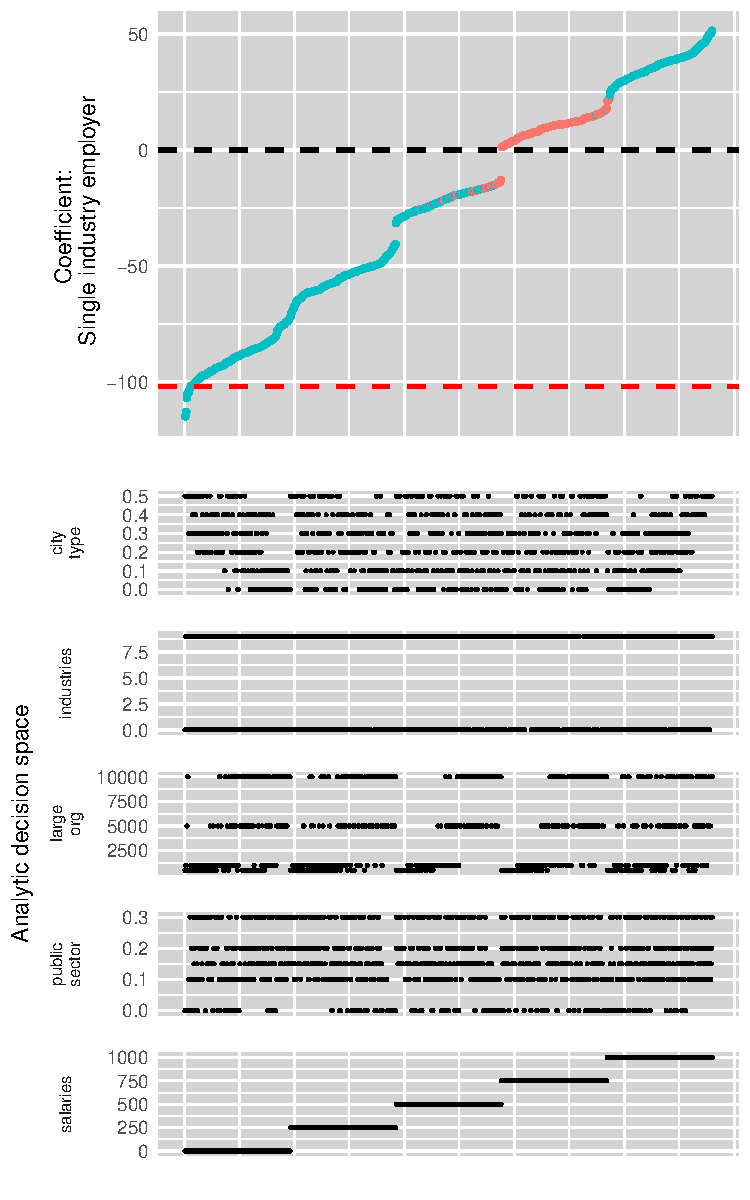
\includegraphics[width=1\textwidth]{1_output_errcorr_singleind.pdf}
   \scalebox{0.55}{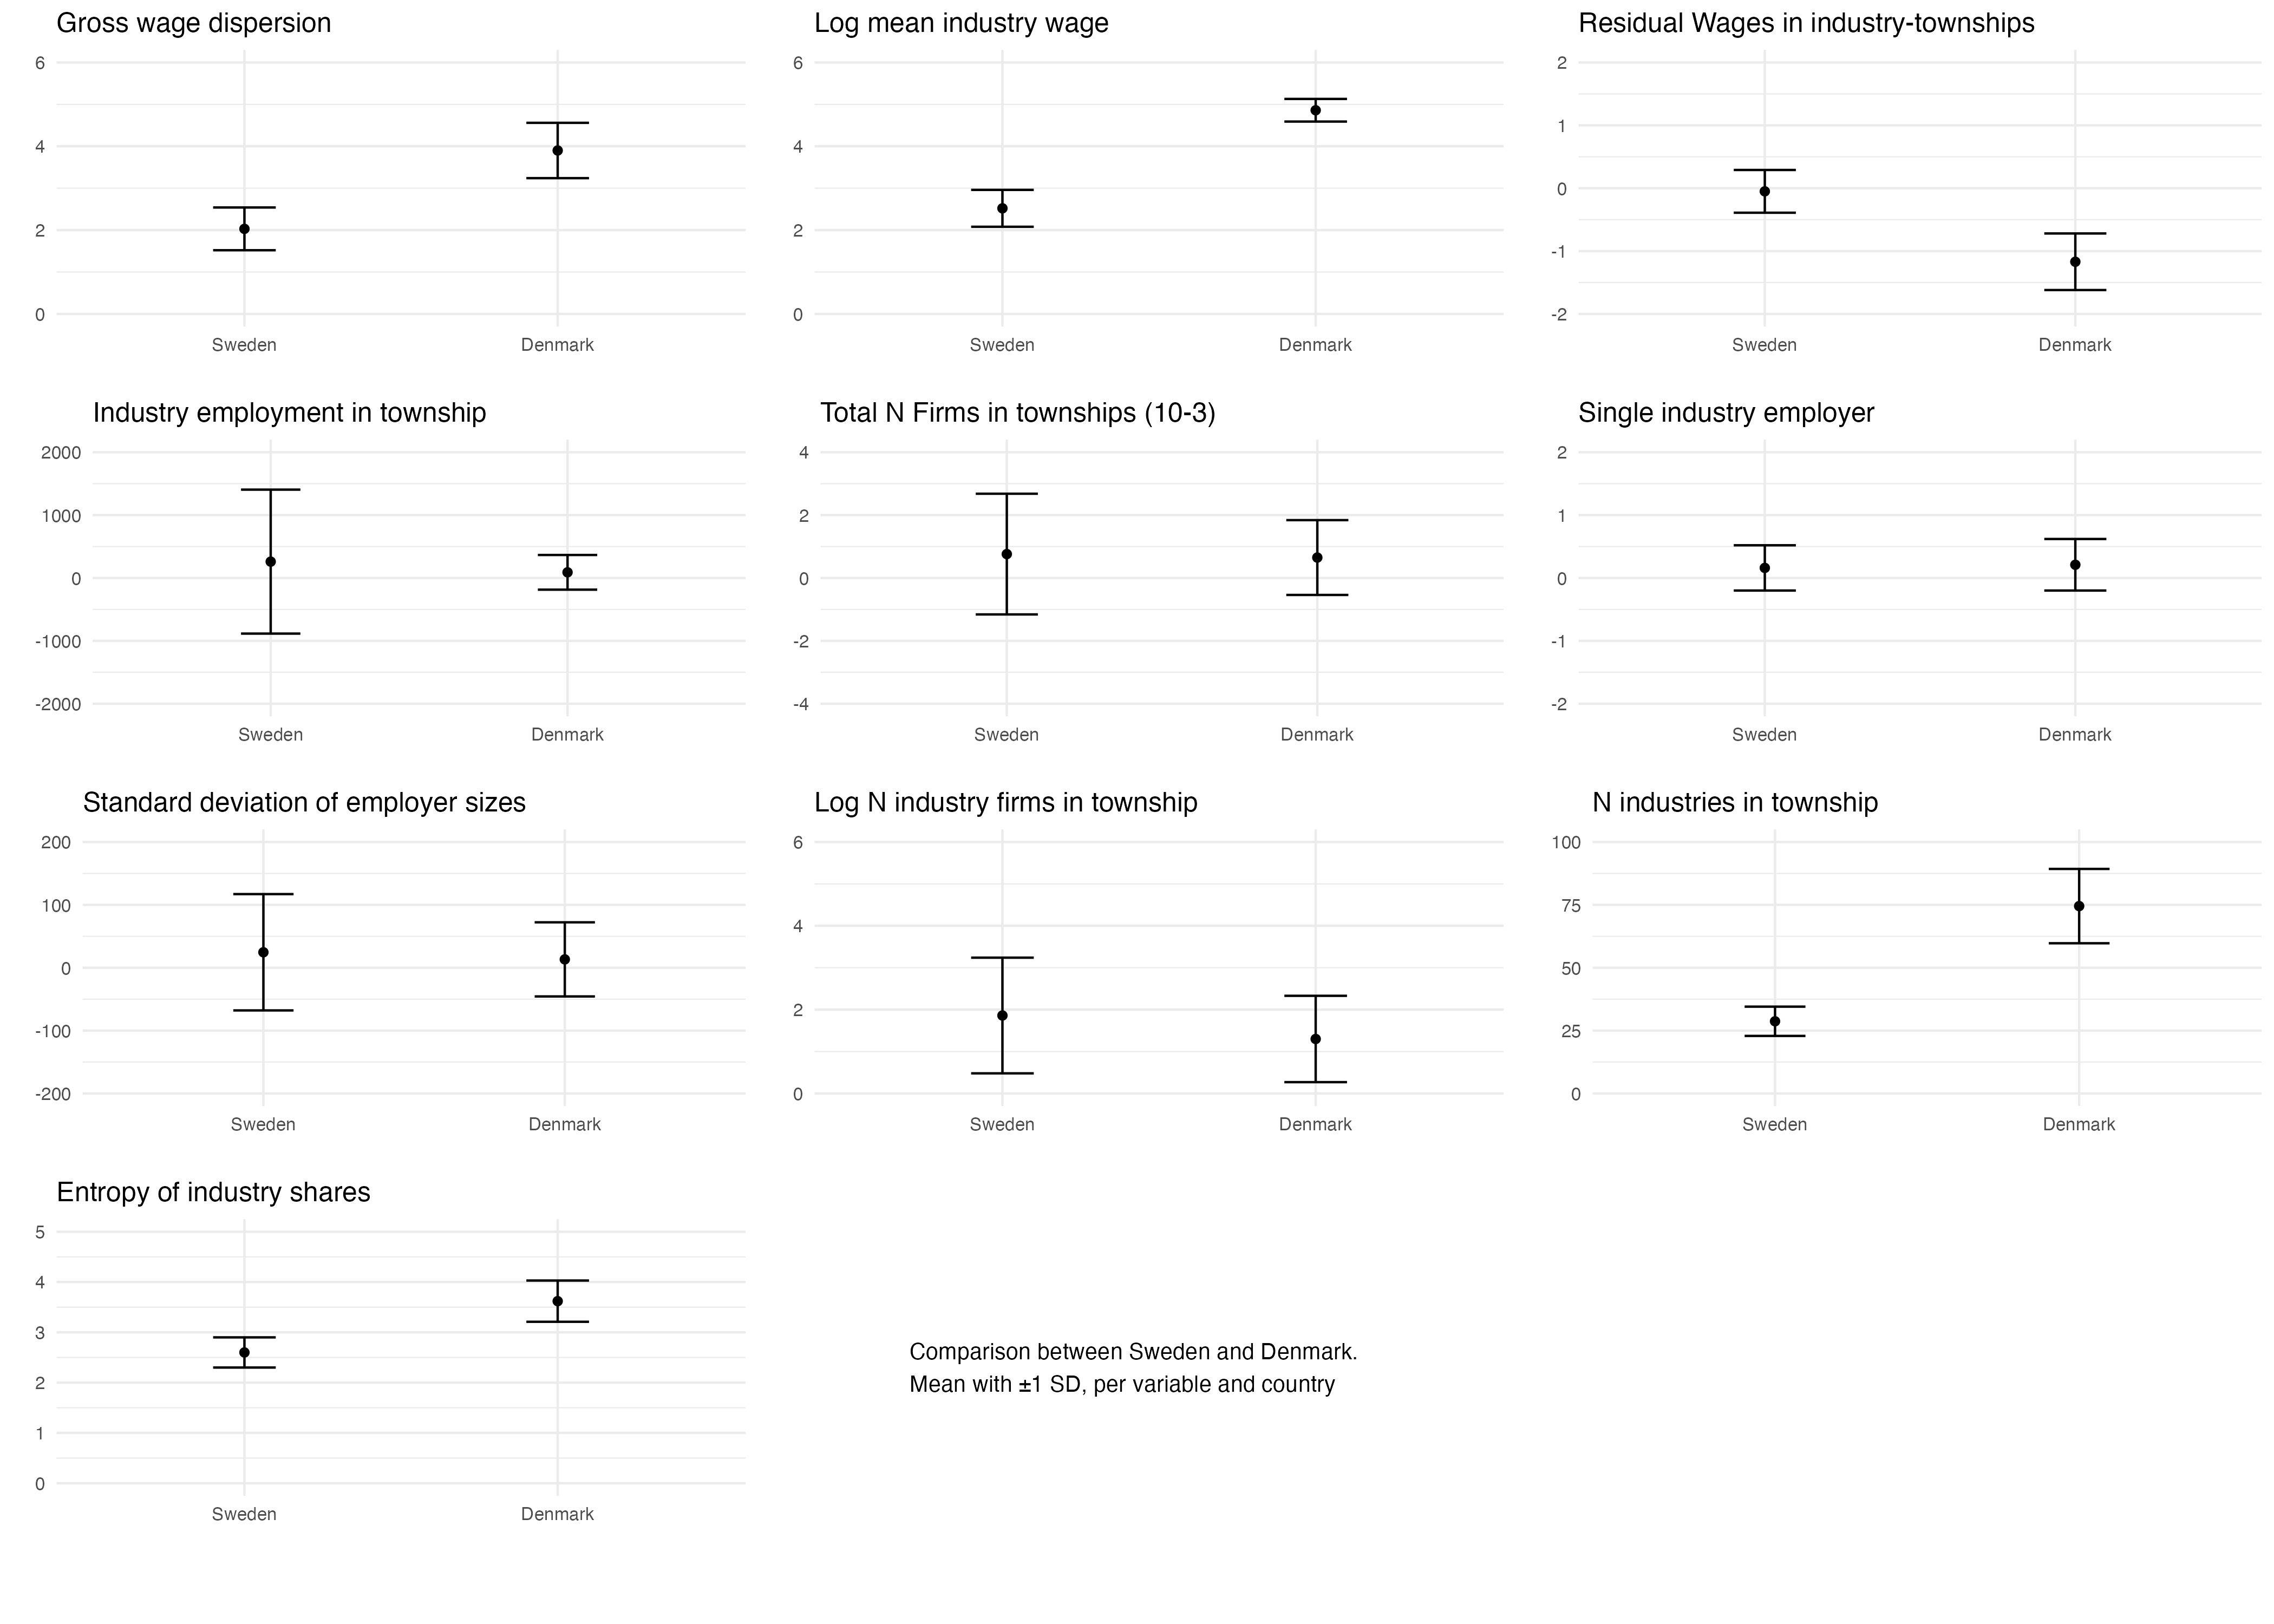
\includegraphics{combined_plot.png}}
    \caption{Comparison of Summary Statistics from Sweden and Denmark, 1992 to 1998. }
  \label{fig:gross_income}
  
\end{figure}
\end{landscape}


%%%%%%%%%%%%%%%%%%%%%%%%%%%
% Multiverse
%%%%%%%%%%%%%%%%%%%%%%%%%%%


\clearpage % Start a new page
%\thispagestyle{empty} % Remove page number from this page

\begin{figure}[htbp]
  \centering
  %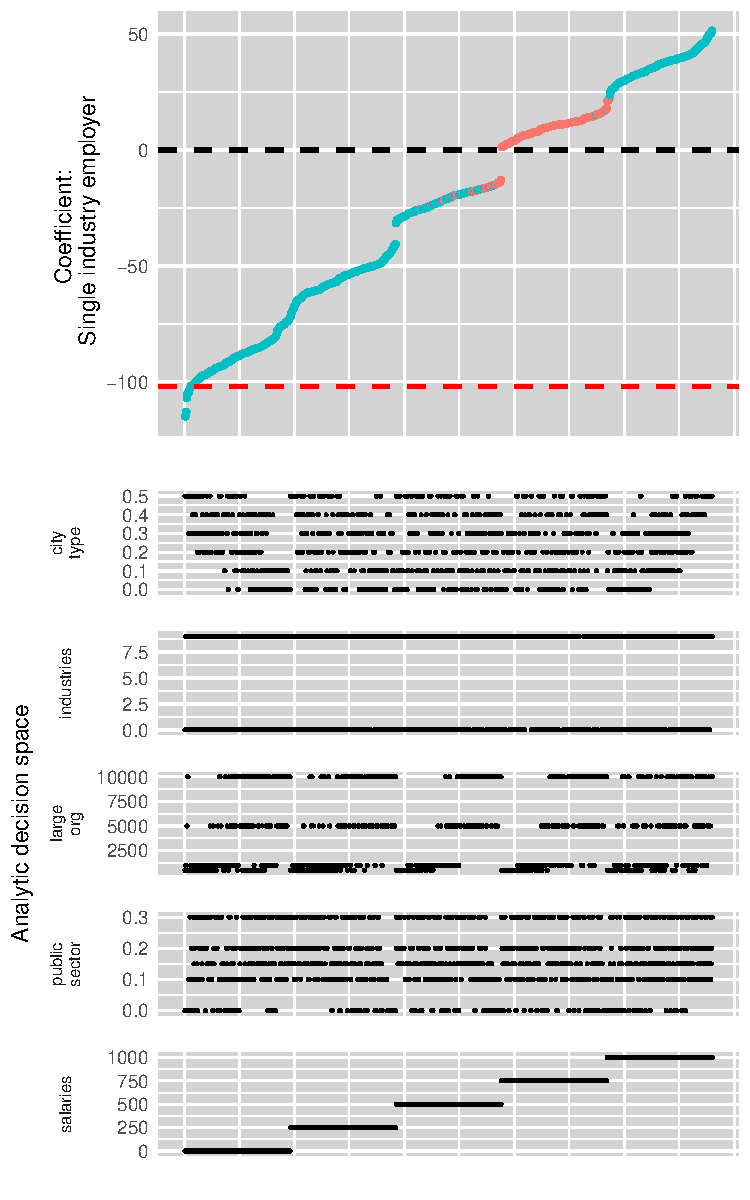
\includegraphics[width=1\textwidth]{1_output_errcorr_singleind.pdf}
   \scalebox{0.85}{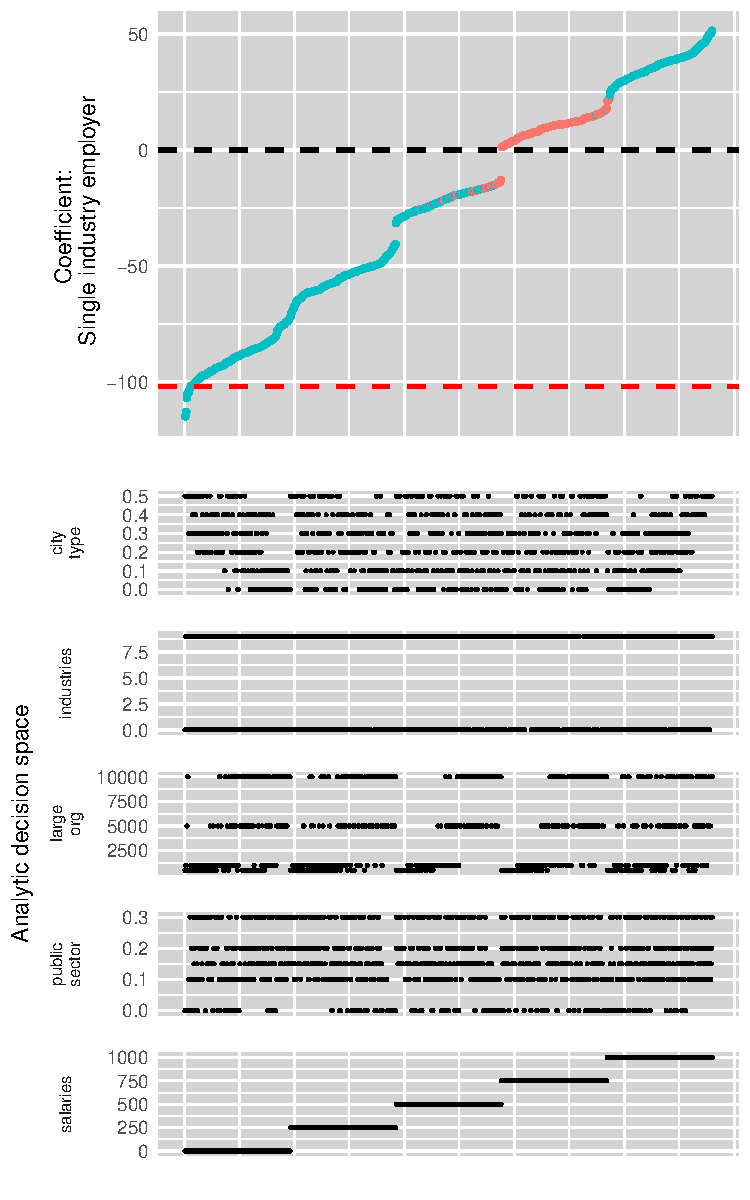
\includegraphics{1_output_errcorr_singleind.pdf}}
    \caption{Specification curves from the multiverse analysis. Estimated Effects of Regional Corporate Demography on Residual Income Dispersion in an Industry-Township, 1992 to 1998.  Single industry employer.}
  \label{fig:gross_income}
  
\end{figure}


\clearpage % Start a new page
%\thispagestyle{empty} % Remove page number from this page


\begin{figure}[htbp]
  \centering
    %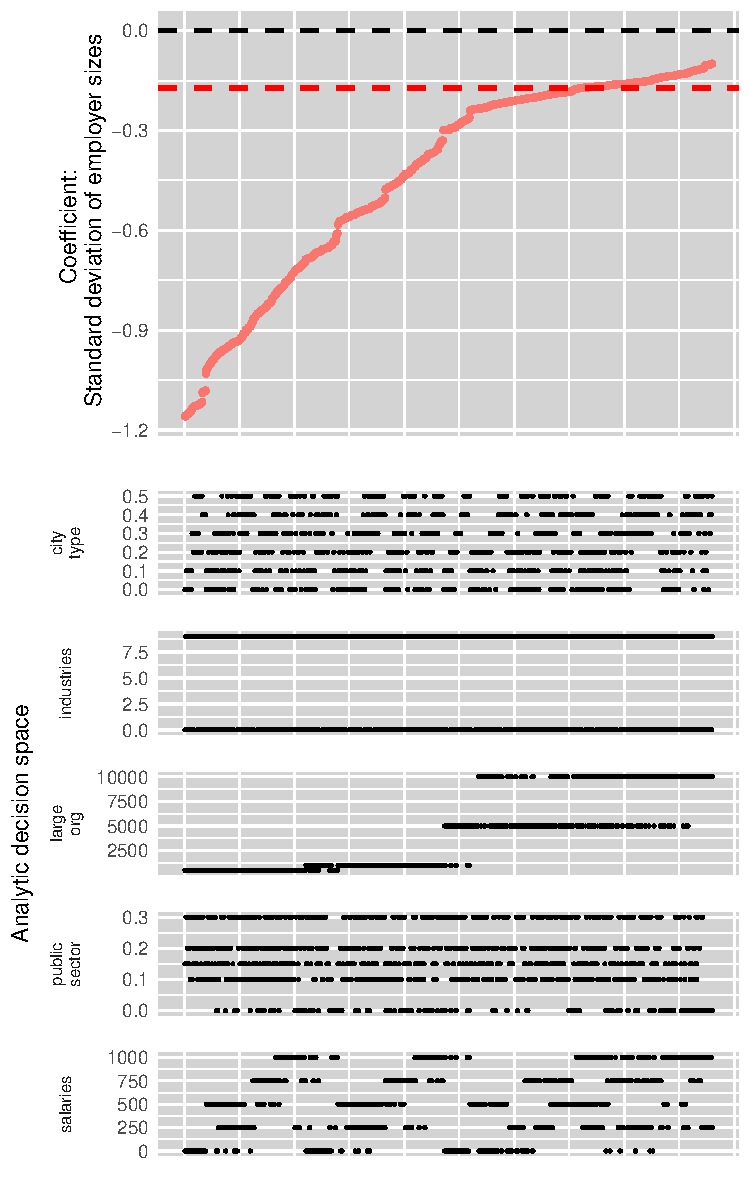
\includegraphics[width=1\textwidth]{2_output_errcorr_sdemployer.pdf}
     \scalebox{0.85}{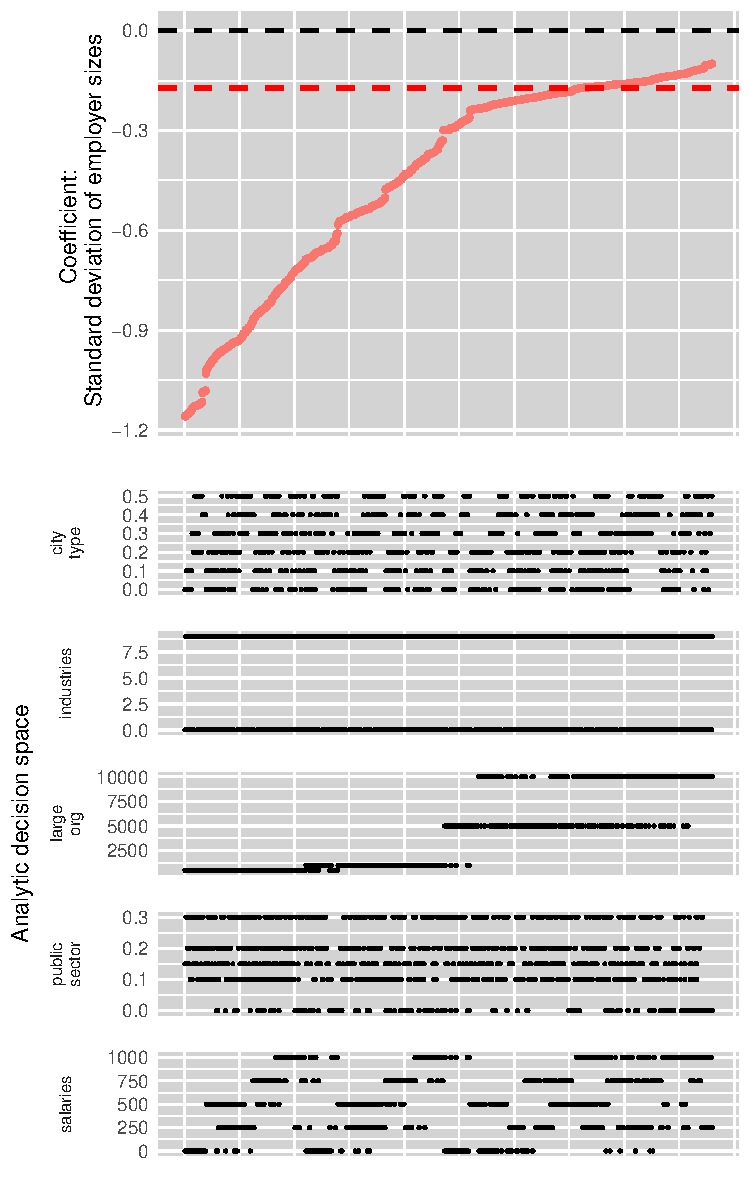
\includegraphics{2_output_errcorr_sdemployer.pdf}}
  \caption{Specification curves from the multiverse analysis. Estimated Effects of Regional Corporate Demography on Residual Income Dispersion in an Industry-Township, 1992 to 1998.  Standard Deviation of Employer Sizes}
  \label{fig:gross_income}
  
\end{figure}

\clearpage % Start a new page
%\thispagestyle{empty} % Remove page number from this page


\begin{figure}[htbp]
  \centering
    %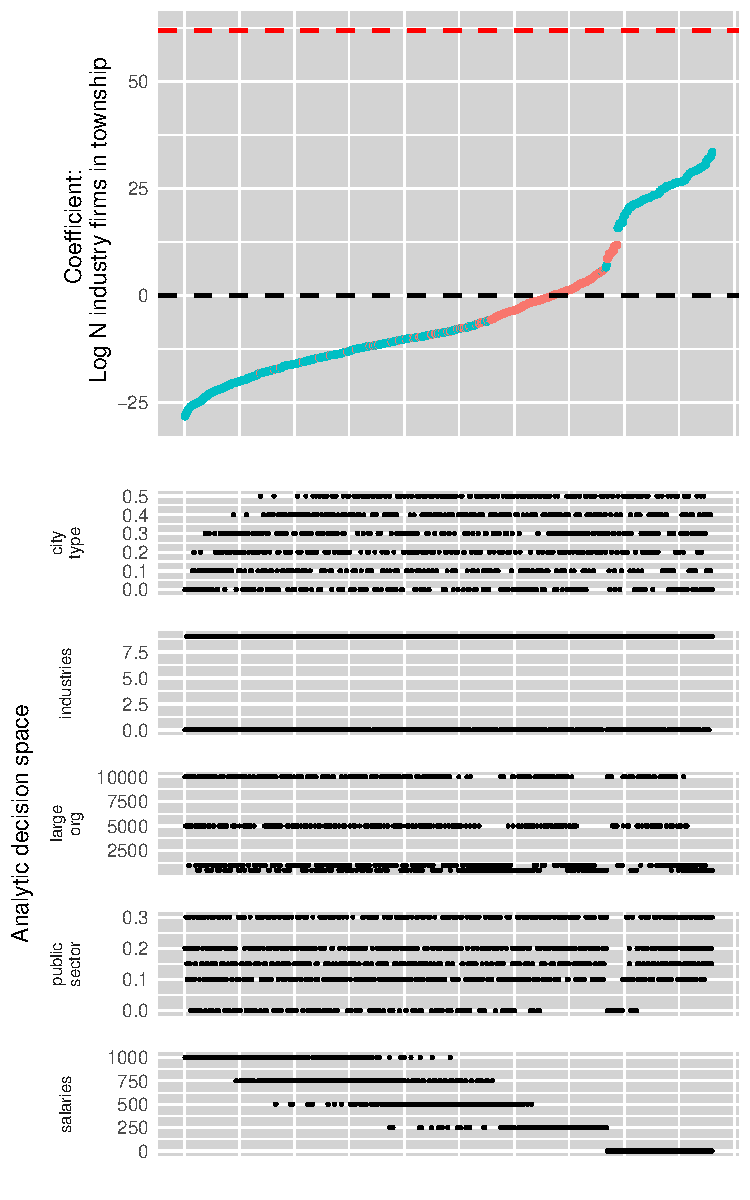
\includegraphics[width=1\textwidth]{3_output_errcorr_log_indfirms.pdf}
     \scalebox{0.85}{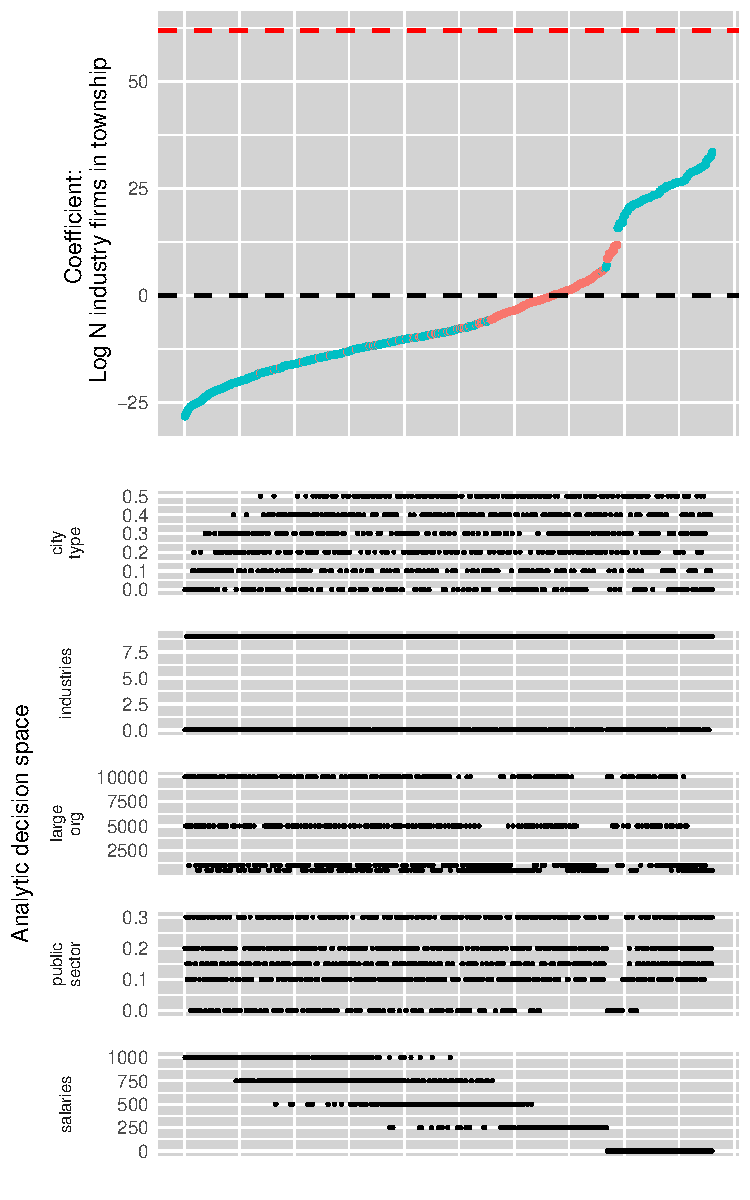
\includegraphics{3_output_errcorr_log_indfirms.pdf}}
  \caption{Specification curves from the multiverse analysis. Estimated Effects of Regional Corporate Demography on Residual Income Dispersion in an Industry-Township, 1992 to 1998.  Log N Industry Firms in Township}
  \label{fig:gross_income}
  
\end{figure}


\clearpage % Start a new page
%\thispagestyle{empty} % Remove page number from this page




\begin{figure}[htbp]
  \centering
    %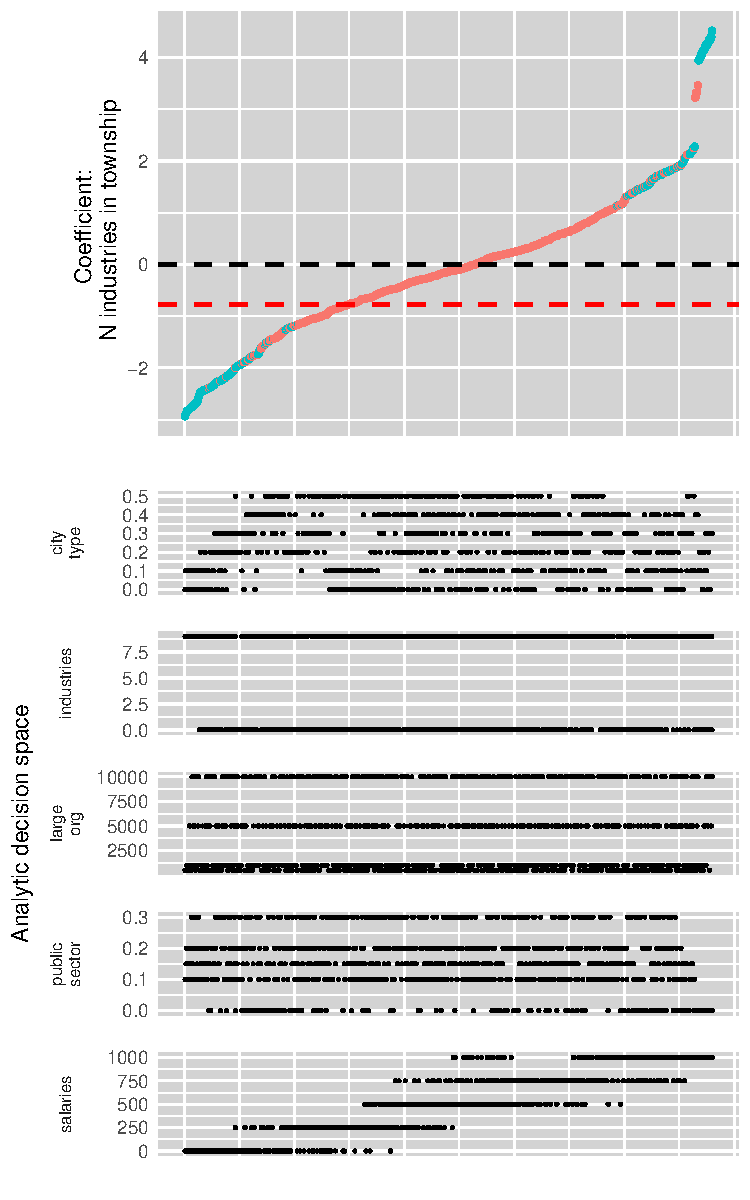
\includegraphics[width=1\textwidth]{4_output_errcorr_nr_ind_in_reg.pdf}
     \scalebox{0.85}{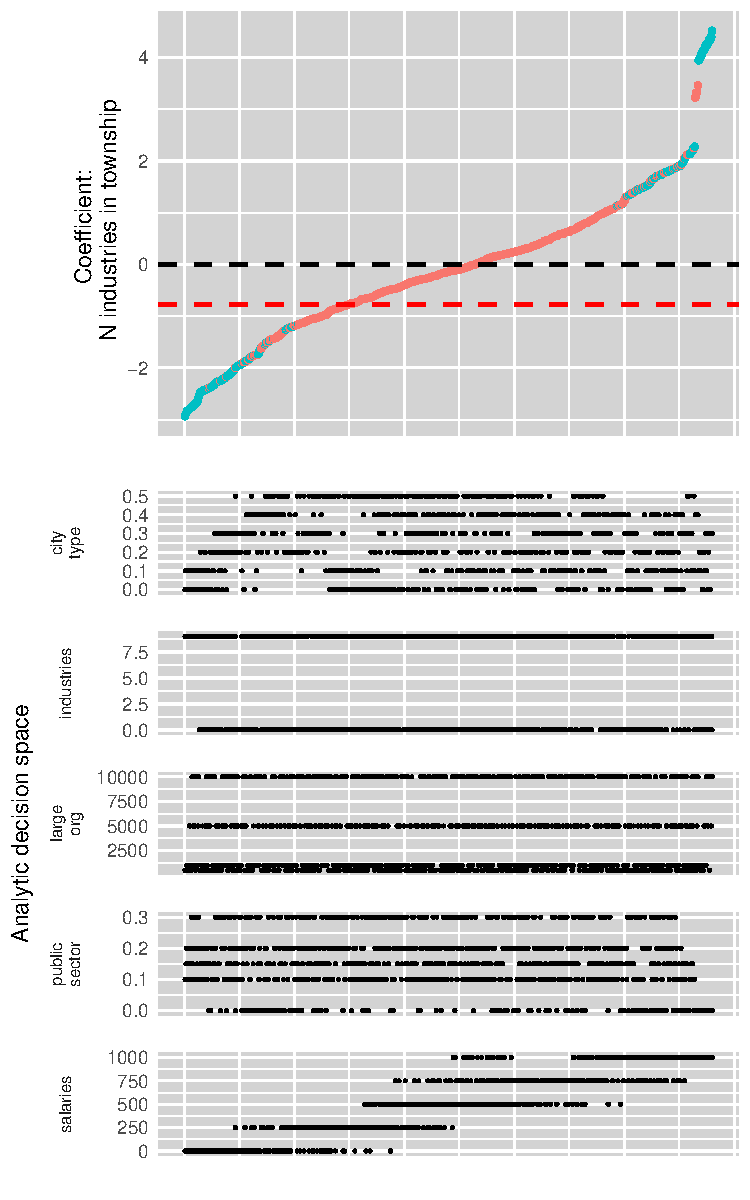
\includegraphics{4_output_errcorr_nr_ind_in_reg.pdf}}
  \caption{Specification curves from the multiverse analysis. Estimated Effects of Regional Corporate Demography on Residual Income Dispersion in an Industry-Township, 1992 to 1998.  N Industries in Township}
  \label{fig:gross_income}
  
\end{figure}


\clearpage % Start a new page
%\thispagestyle{empty} % Remove page number from this page

\begin{figure}[htbp]
  \centering
    %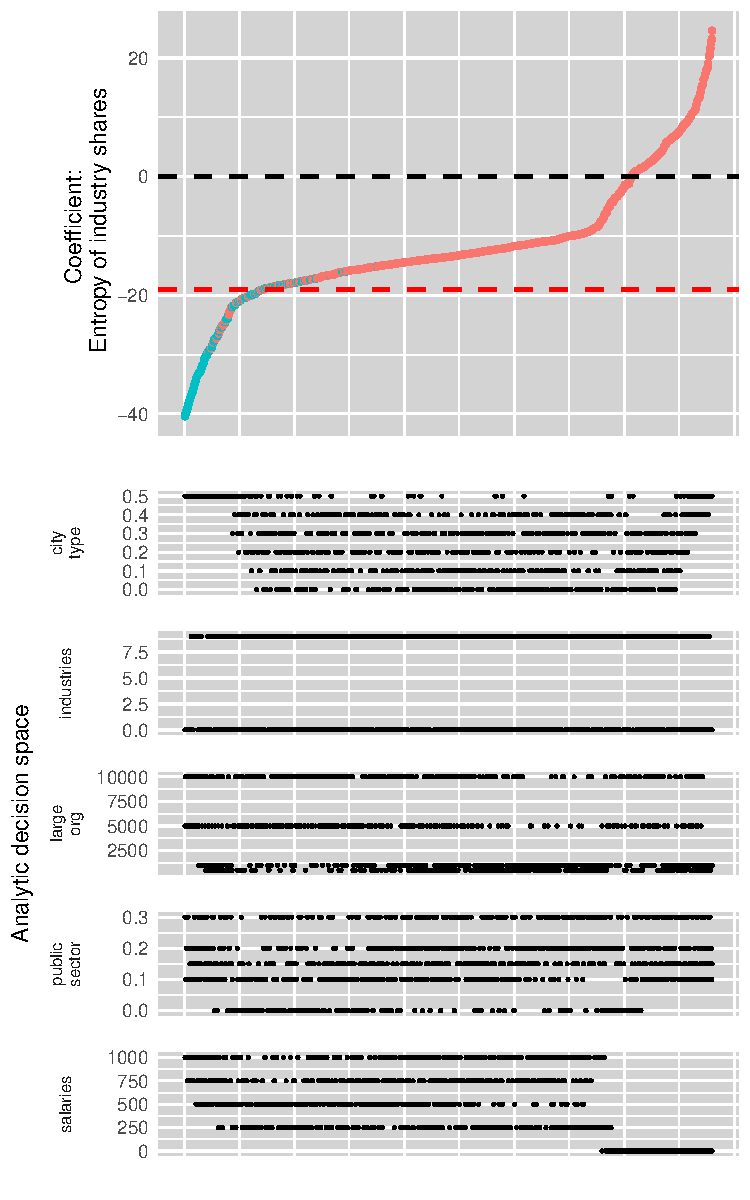
\includegraphics[width=1\textwidth]{5_output_errcorr_ent.pdf}
     \scalebox{0.85}{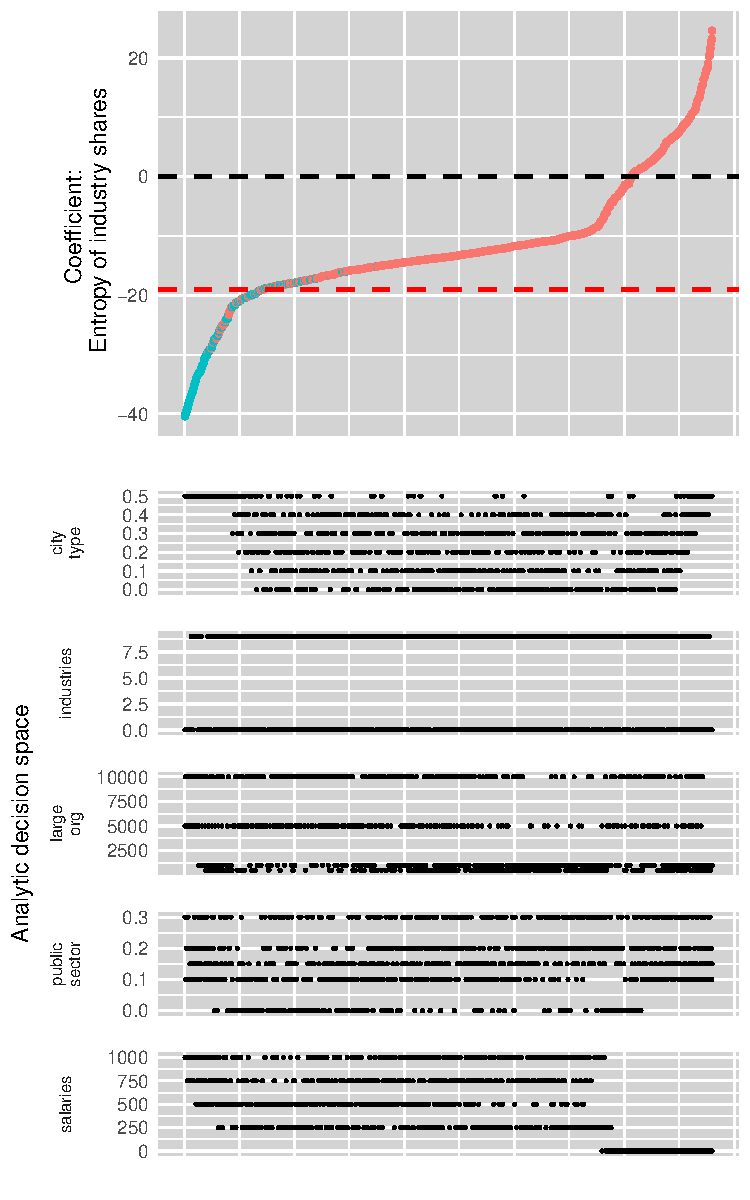
\includegraphics{5_output_errcorr_ent.pdf}}
  \caption{Specification curves from the multiverse analysis. Estimated Effects of Regional Corporate Demography on Residual Income Dispersion in an Industry-Township, 1992 to 1998.  Entropy of Industry Shares}
  \label{fig:gross_income}
  
\end{figure}



\clearpage % Start a new page
%\thispagestyle{empty} % Remove page number from this page

\begin{figure}[htbp]
  \centering
    %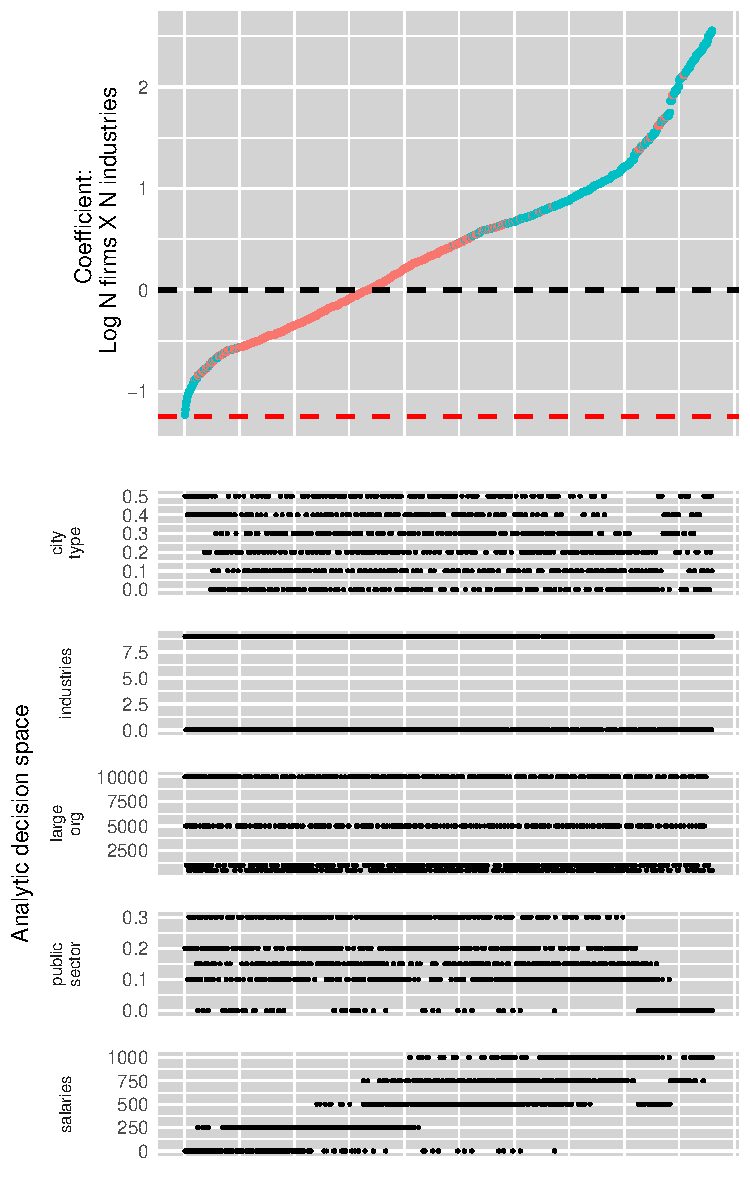
\includegraphics[width=1\textwidth]{6_output_errcorr_indfirmXindreg.pdf}
     \scalebox{0.85}{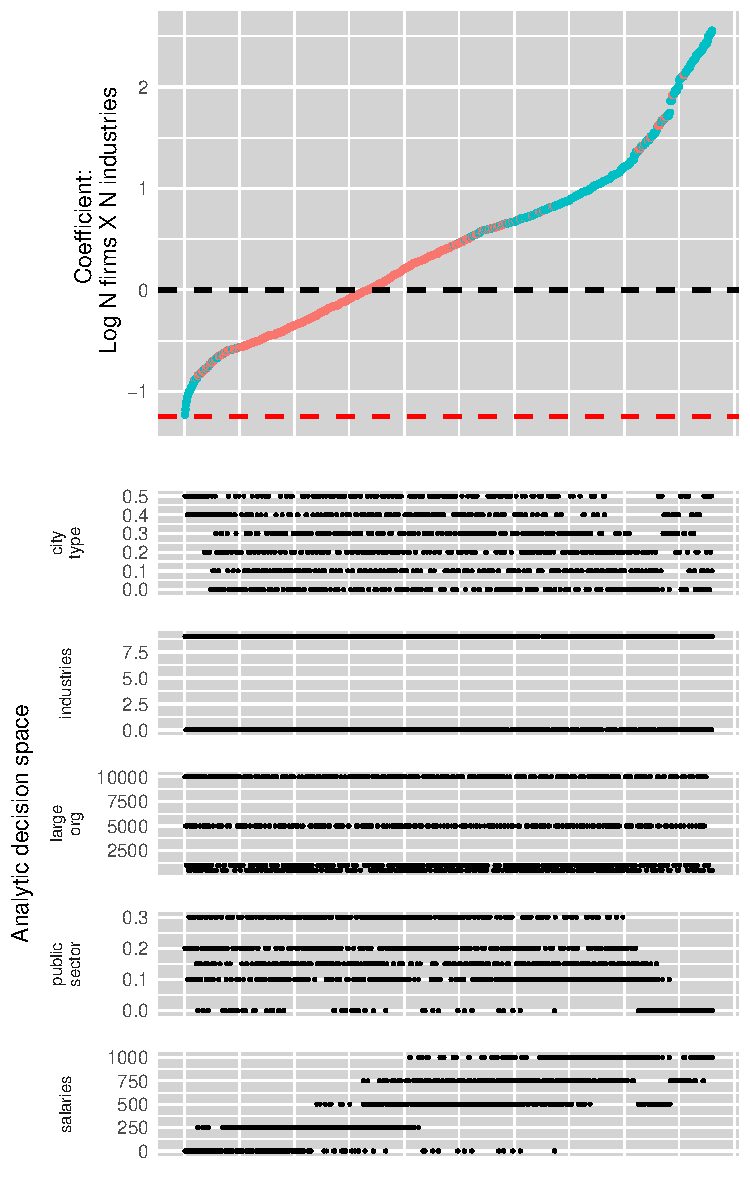
\includegraphics{6_output_errcorr_indfirmXindreg.pdf}}
  \caption{Specification curves from the multiverse analysis. Estimated Effects of Regional Corporate Demography on Residual Income Dispersion in an Industry-Township, 1992 to 1998.  Log N Firms X N Industries}
  \label{fig:gross_income}
  
\end{figure}


\clearpage % Start a new page
%\thispagestyle{empty} % Remove page number from this page

\begin{figure}[htbp]
  \centering
   % 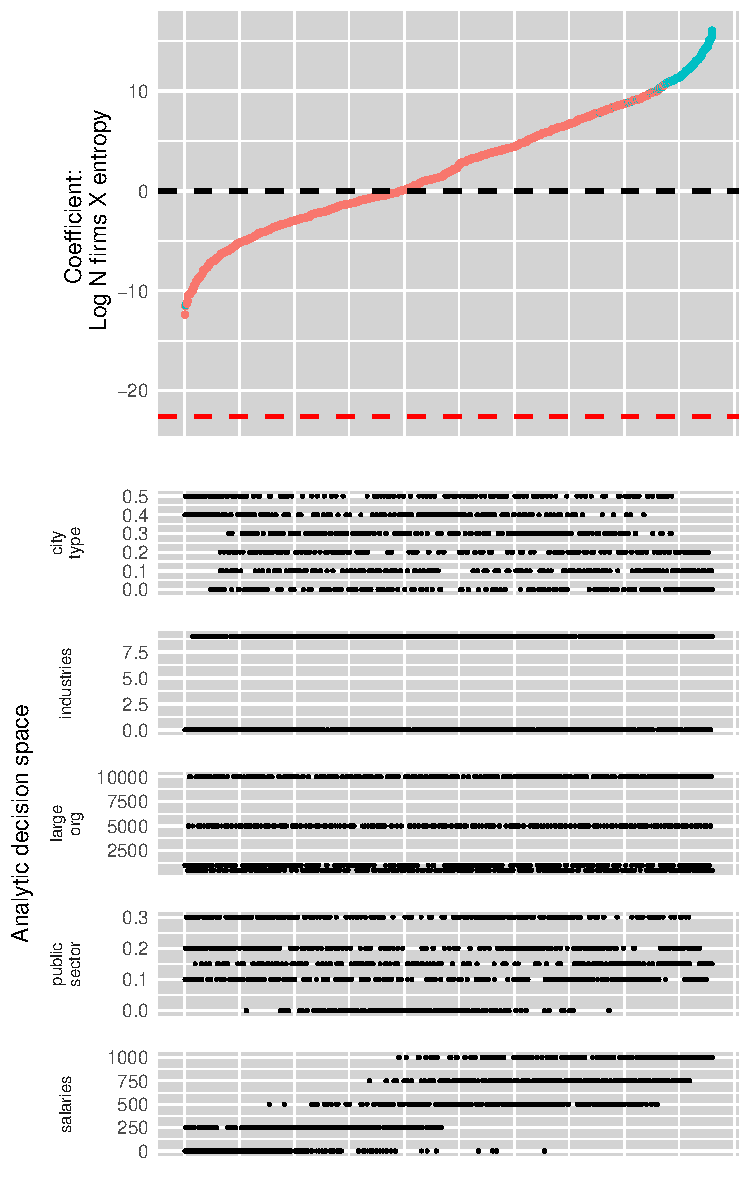
\includegraphics[width=1\textwidth]{7_output_errcorr_indfirmXent.pdf}
     \scalebox{0.85}{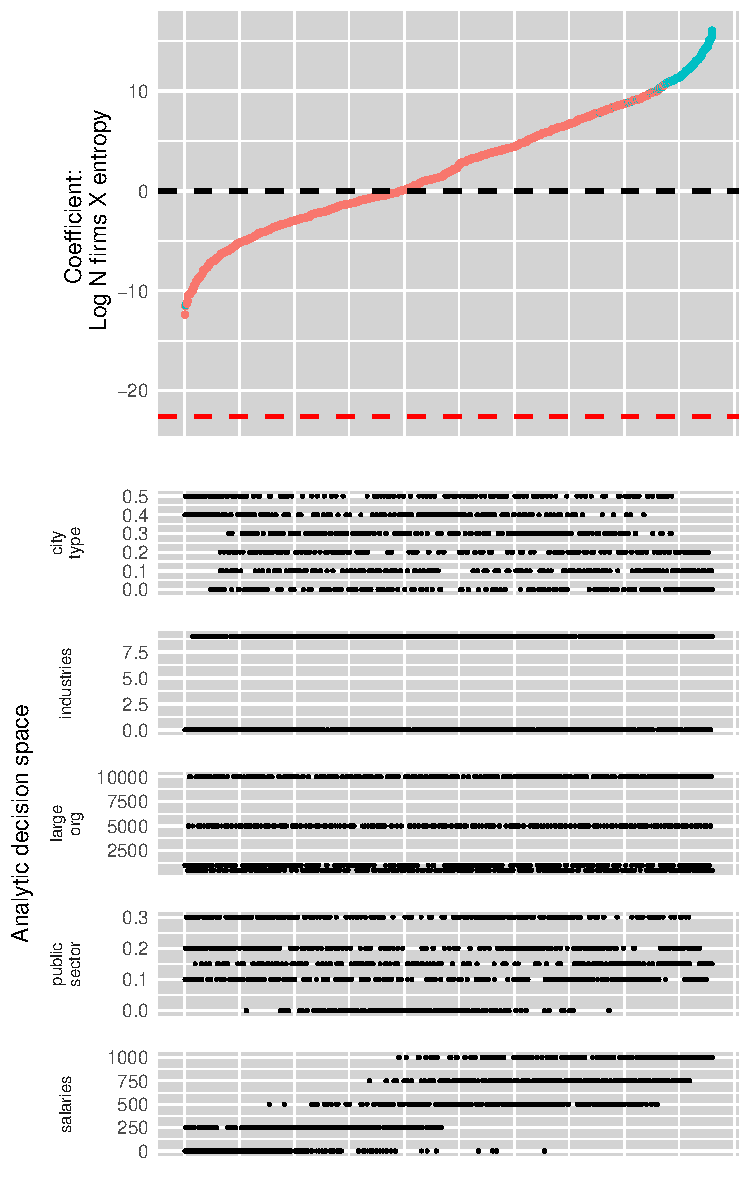
\includegraphics{7_output_errcorr_indfirmXent.pdf}}
  \caption{Specification curves from the multiverse analysis. Estimated Effects of Regional Corporate Demography on Residual Income Dispersion in an Industry-Township, 1992 to 1998.  Log N Firms X Entropy}
  \label{fig:gross_income}
  
\end{figure}


%%  \scalebox{0.9}{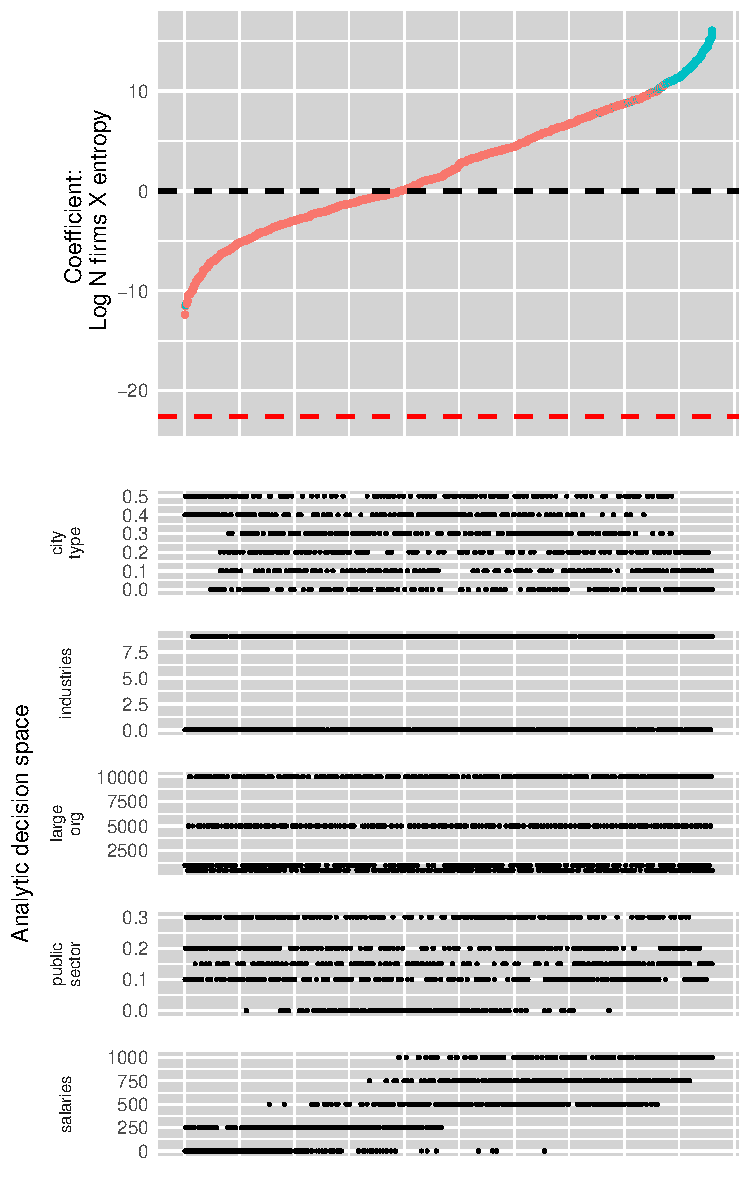
\includegraphics{7_output_errcorr_indfirmXent.pdf}}





\end{document}